\documentclass[hyperref=colorlinks]{beamer}
\mode<presentation>
\usetheme{iclpt}
\setbeamertemplate{navigation symbols}{}
\setbeamertemplate{headline}{
  \begin{beamercolorbox}[leftskip=.2cm,rightskip=.2cm,topskip=.2cm,ht=1.1cm,dp=0.1cm,wd=\textwidth]{institute in head/foot}
    
\includegraphics[height=1cm]{icl.pdf}
    \hfill
%    \includegraphics[height=1cm]{../Pics/ATLAS-Logo-Square-Blue-RGB.png}
%    
\includegraphics[height=1cm]{../Pics/CMS-Color.pdf}
    
\includegraphics[height=1cm]{TalkPics/t2k_logo_large.png}

%??put t2k logo here
  \end{beamercolorbox}
}
\setbeamertemplate{footline}{
  \begin{beamercolorbox}[ht=.35cm,dp=0.2cm,wd=\textwidth,leftskip=.3cm]{author in head/foot}%
    \begin{minipage}[c]{5cm}%
      \usebeamerfont{author in head/foot}
      \insertshortauthor 
      \insertshorttitle
    \end{minipage}\hfill%
    \hfill
    \insertframenumber{} / \ref{lastframe}
    %\hfill
    \begin{minipage}{6cm}
      \hfill
      %\insertshorttitle
    \end{minipage}
  \end{beamercolorbox}%
}

\definecolor{beamer@icdarkblue}{RGB}{0,51,102}
\definecolor{beamer@icmiddleblue}{RGB}{0,82,150} 
\definecolor{beamer@iclightblue}{RGB}{200,212,232}
\definecolor{beamer@icmiddlered}{RGB}{204,51,0}
\definecolor{beamer@iclightred}{RGB}{232,212,32}

\usepackage{tikz}
\usetikzlibrary{arrows,shapes,backgrounds}
\usepackage{color}
\usepackage{tabularx,colortbl}
\usepackage{graphicx}
\usepackage{pdfpages}
\usepackage{feynmp}
\usepackage{rotating}
\usepackage{moresize}
\usepackage{slashed}
\usepackage{xcolor,colortbl}
\DeclareGraphicsRule{*}{mps}{*}{}
\hypersetup{colorlinks=false}

\title[2D vs 1D yields]{\vspace{-0.2cm} Status Report for Run 1-7c joint fit Update}
\author[P. Dunne]{Patrick Dunne - Imperial College London}
\titlegraphic{
  \vspace{-0.4cm}
}
\date{}
\begin{document}
\tikzstyle{every picture}+=[remember picture]
\tikzstyle{na} = [baseline=-.5ex]
\begin{fmffile}{t2ktemplatefeyndiags}


  %TITLE PAGE
  %20 mins + 5 questions
  \section{Title}
  \begin{frame}
    \titlepage
  \end{frame}

  \begin{frame}
    \frametitle{Overview}
    \begin{block}{}
      \scriptsize
      \begin{itemize}
      \item All three analyses are updating to the full Run 1-7c dataset
      \item[-] FHC POT: $7.48\times10^{20}$ RHC POT: $7.47\times10^{20}$
      \item Working to get the joint fit ready by ICHEP
      \item Asimov rates have been compared and found to be in good agreement
      \item Will show comparisons between the three groups asimov contours and first data results today
      \item[-] All results are with reactor constraint
      \end{itemize}
    \end{block}
  \end{frame}

  \begin{frame}
    \centering
    \huge \textcolor{beamer@icmiddleblue}{Asimov comparisons}
  \end{frame}

  \begin{frame}
    \frametitle{Comparison of Asimov Set 1 2D contours - NH}
    \centering
    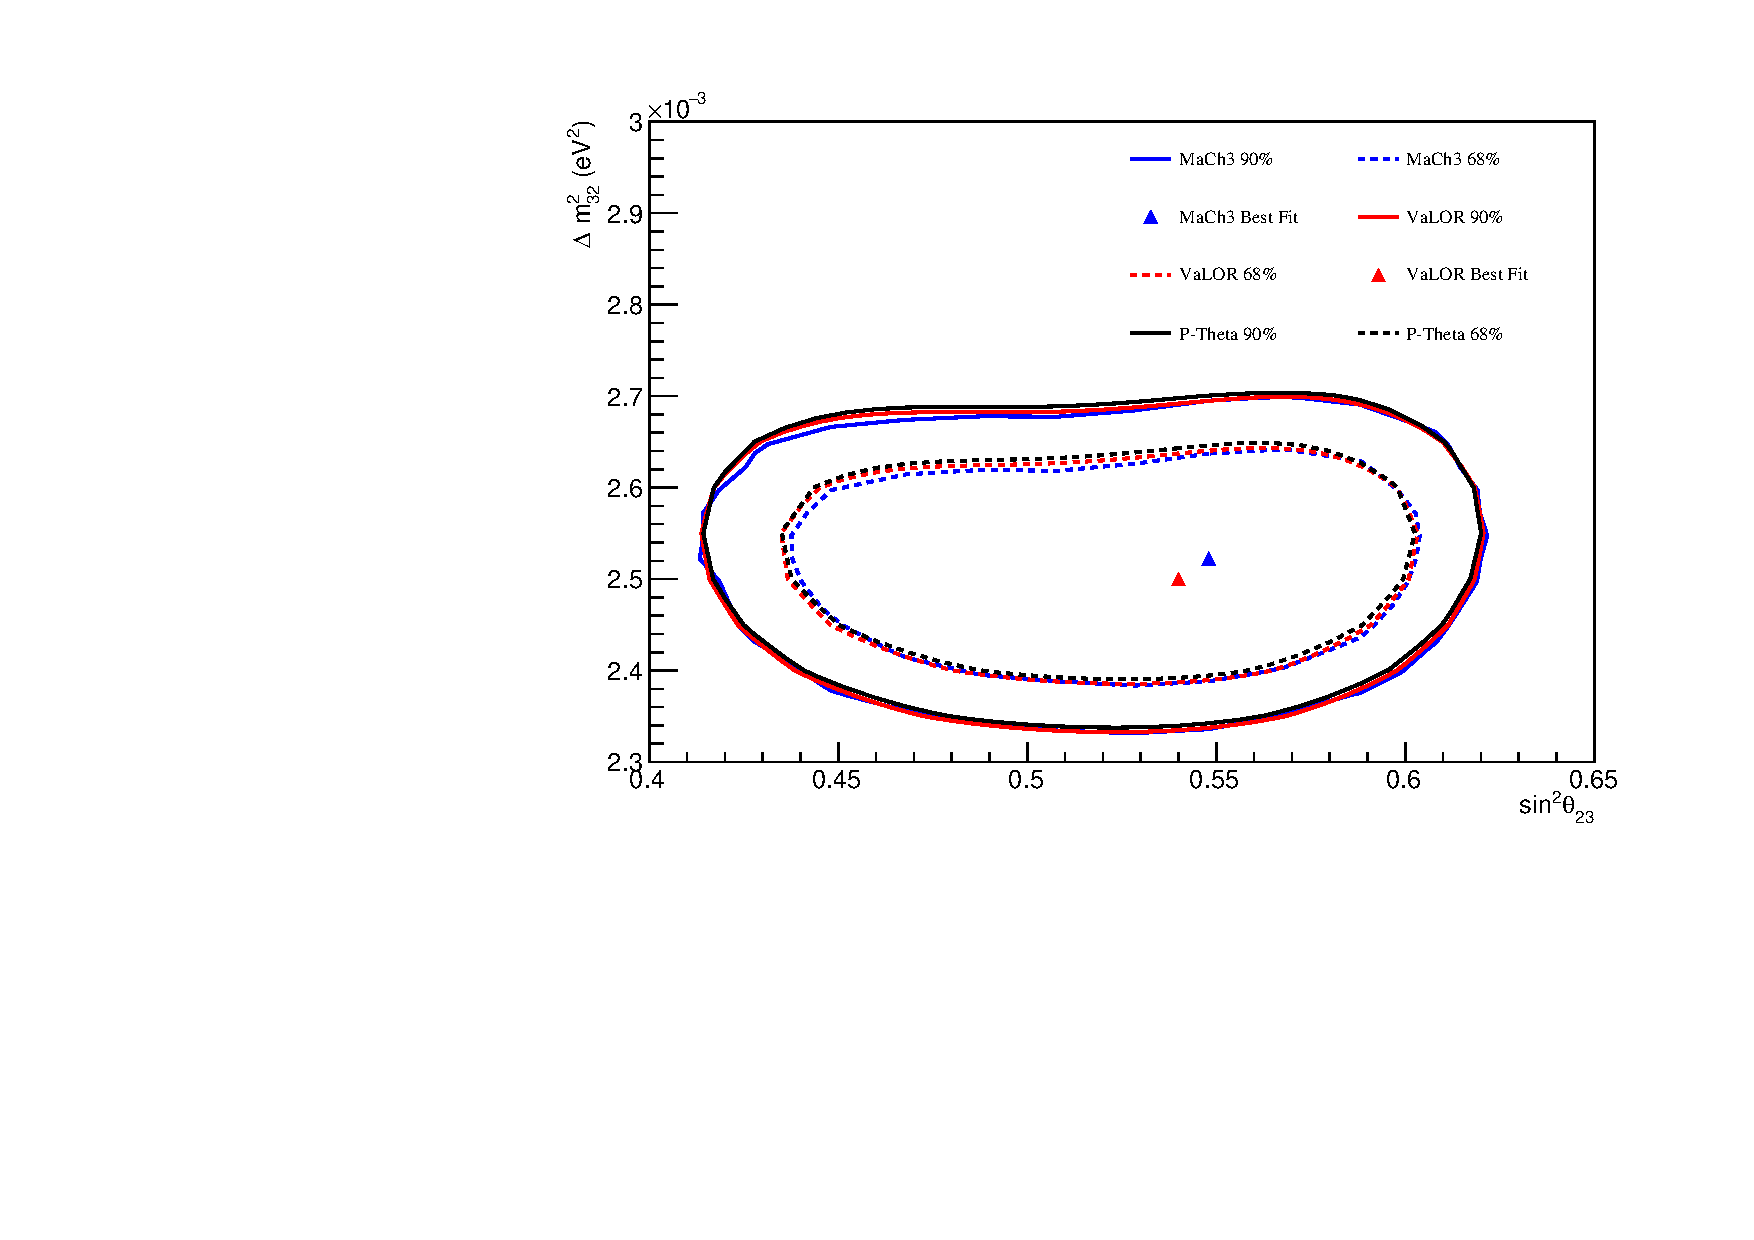
\includegraphics[width=.8\textwidth]{TalkPics/run17canalysescomparisons_210716/comparedcontours/comparedcontours_threeanalyses_NH.pdf}
  \end{frame}

  \begin{frame}
    \frametitle{Comparison of Asimov Set 1 2D contours - IH}
    \centering
    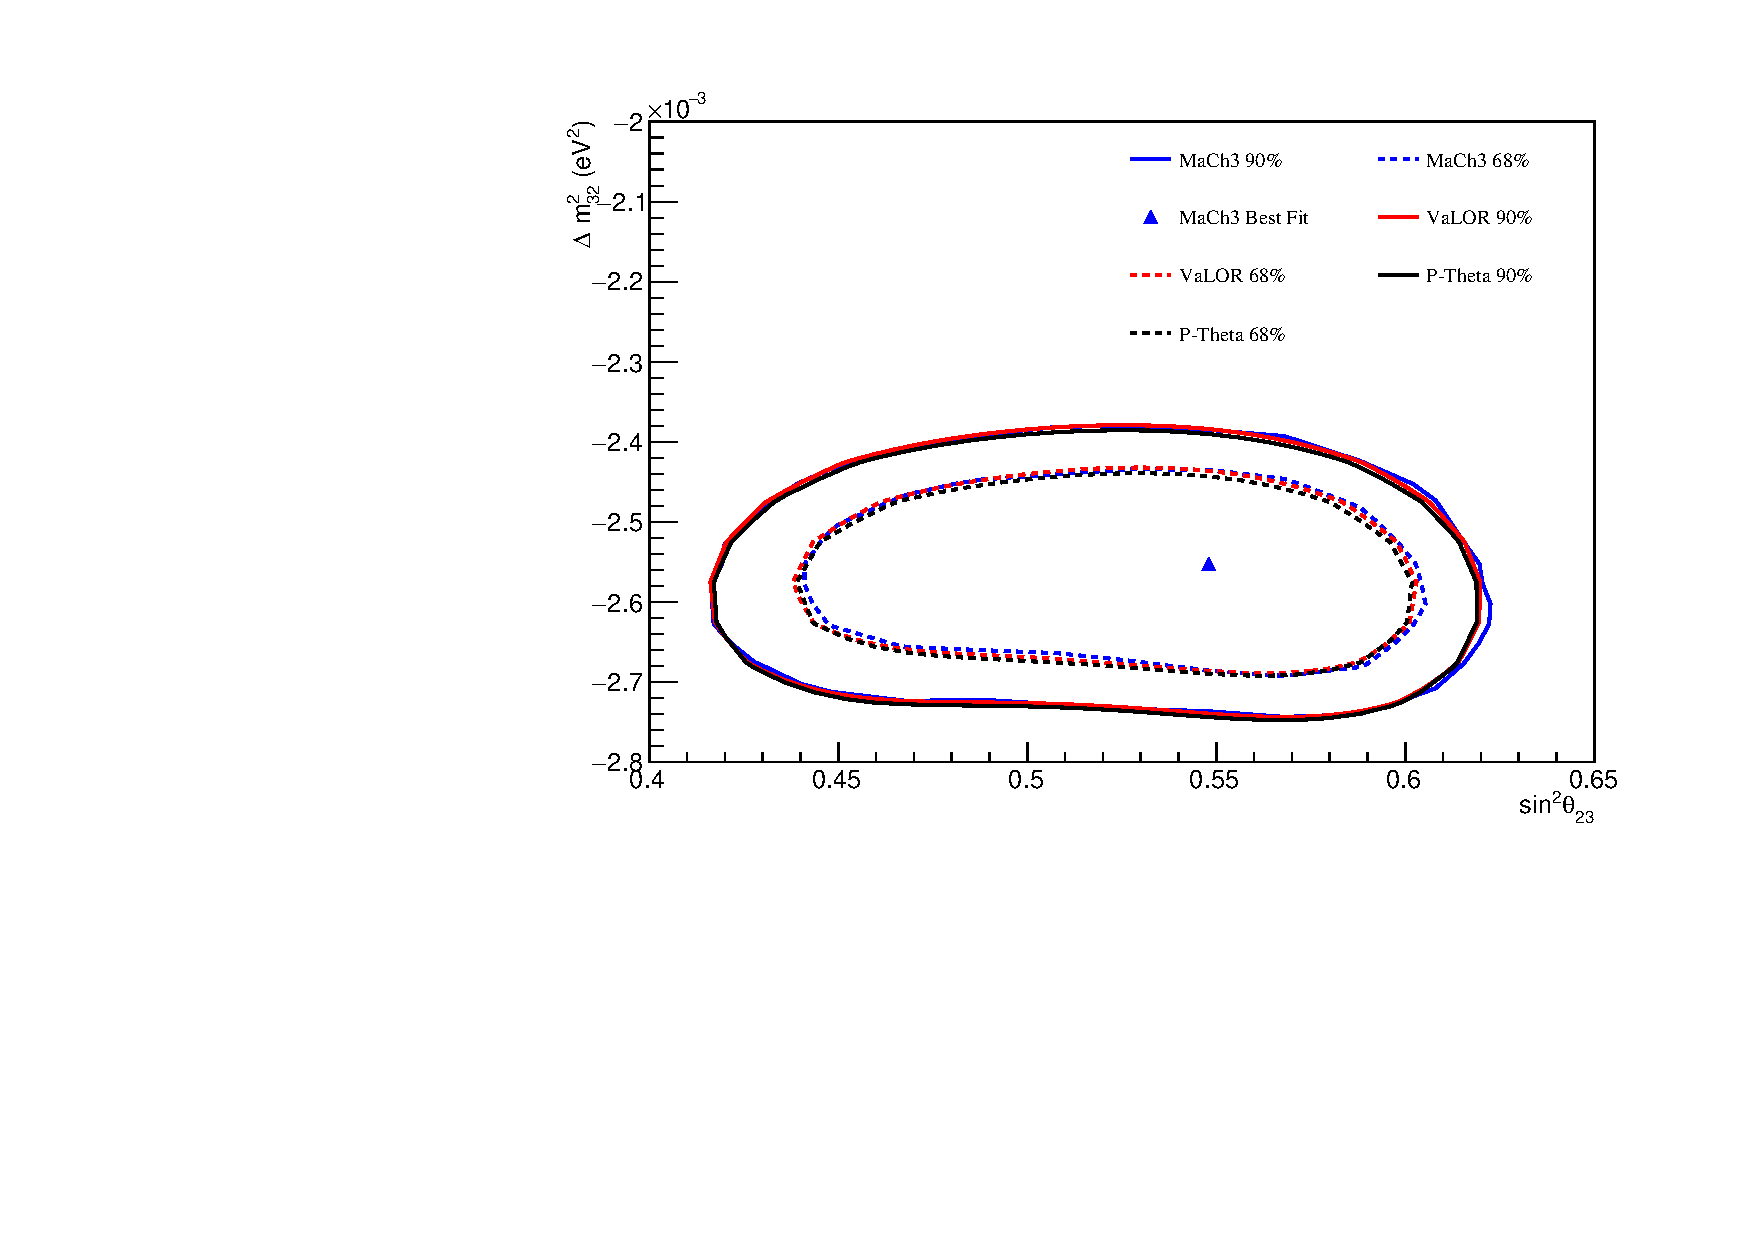
\includegraphics[width=.8\textwidth]{TalkPics/run17canalysescomparisons_210716/comparedcontours/comparedcontours_threeanalyses_IH.pdf}
  \end{frame}

  \begin{frame}
    \frametitle{Comparison of Asimov Set 1 2D contours - NH}
    \centering
    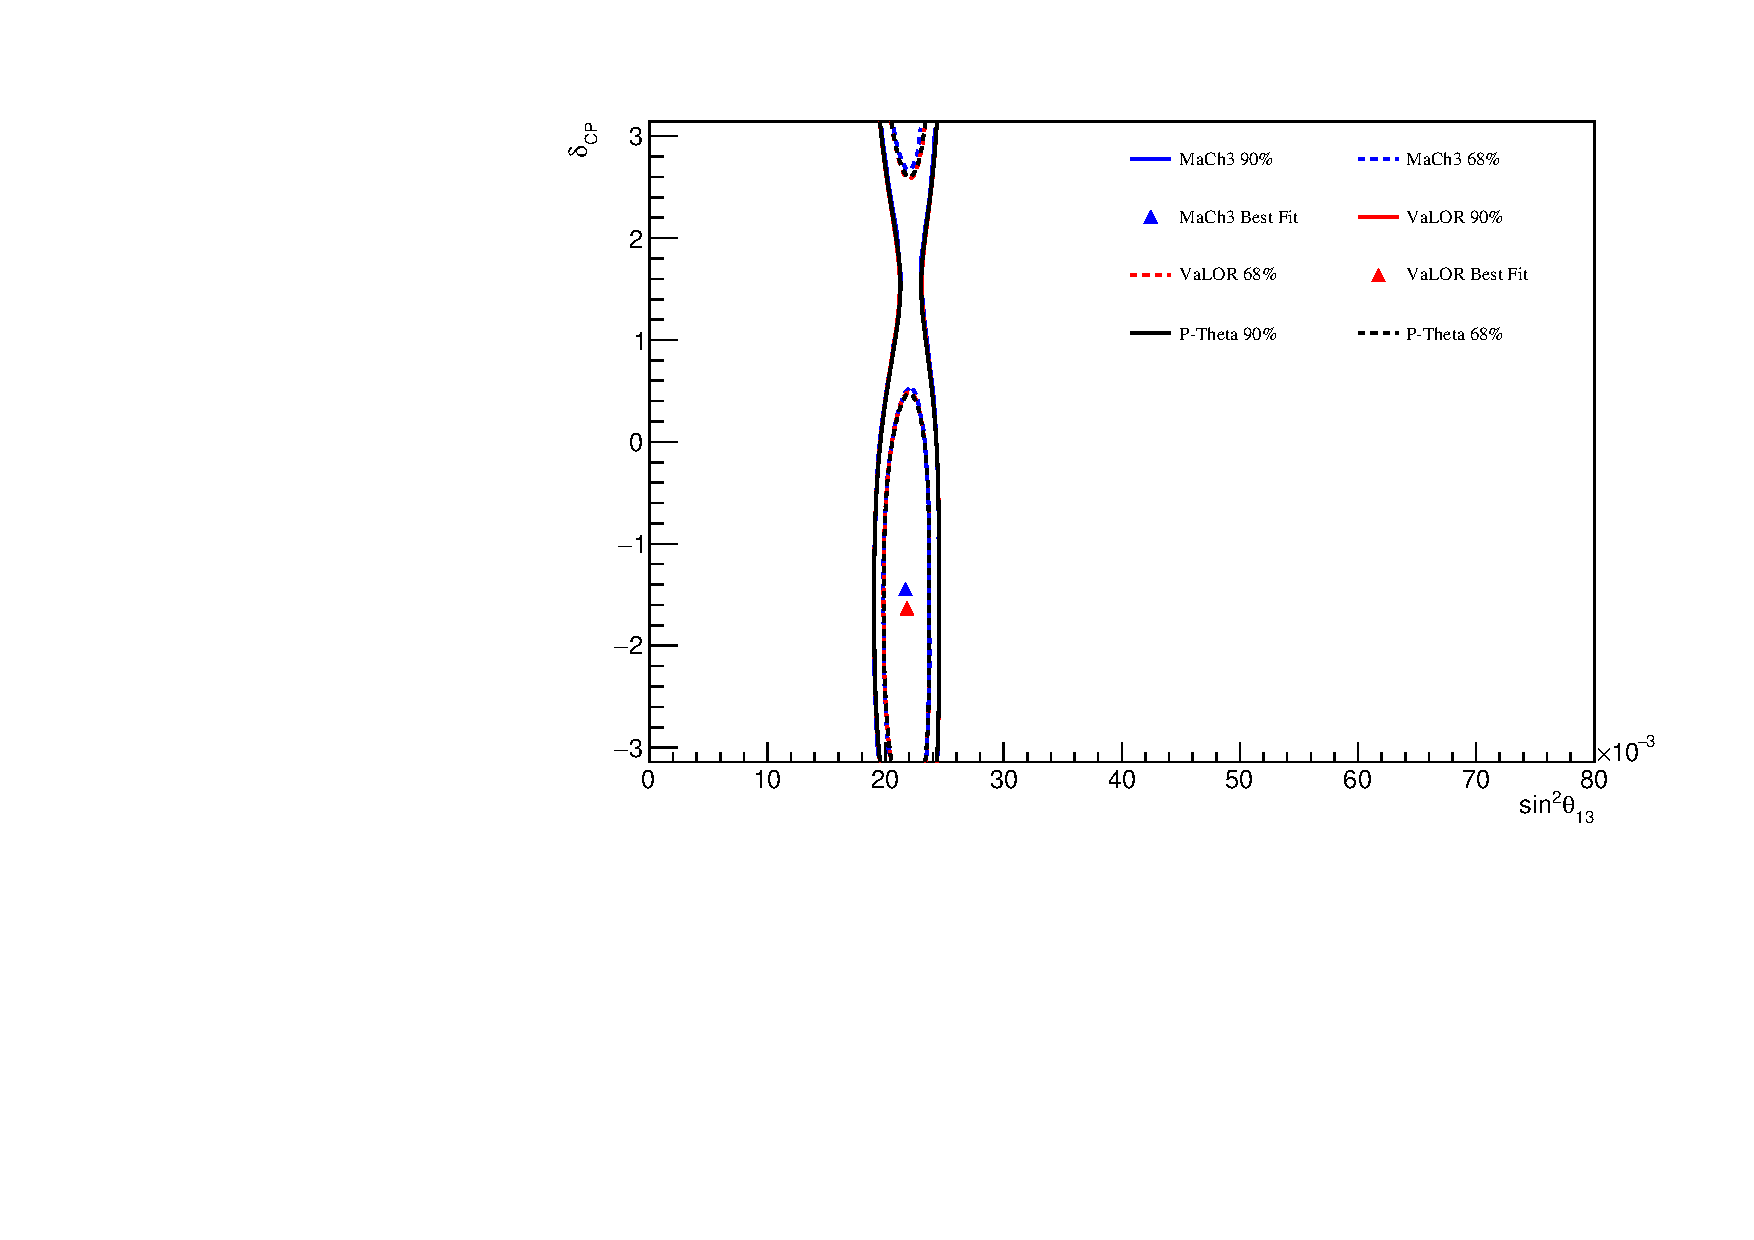
\includegraphics[width=.8\textwidth]{TalkPics/run17canalysescomparisons_210716/comparedcontours/comparedcontours_threeanalyses_th13dcp_NH.pdf}
  \end{frame}

  \begin{frame}
    \frametitle{Comparison of Asimov Set 1 2D contours - IH}
    \centering
    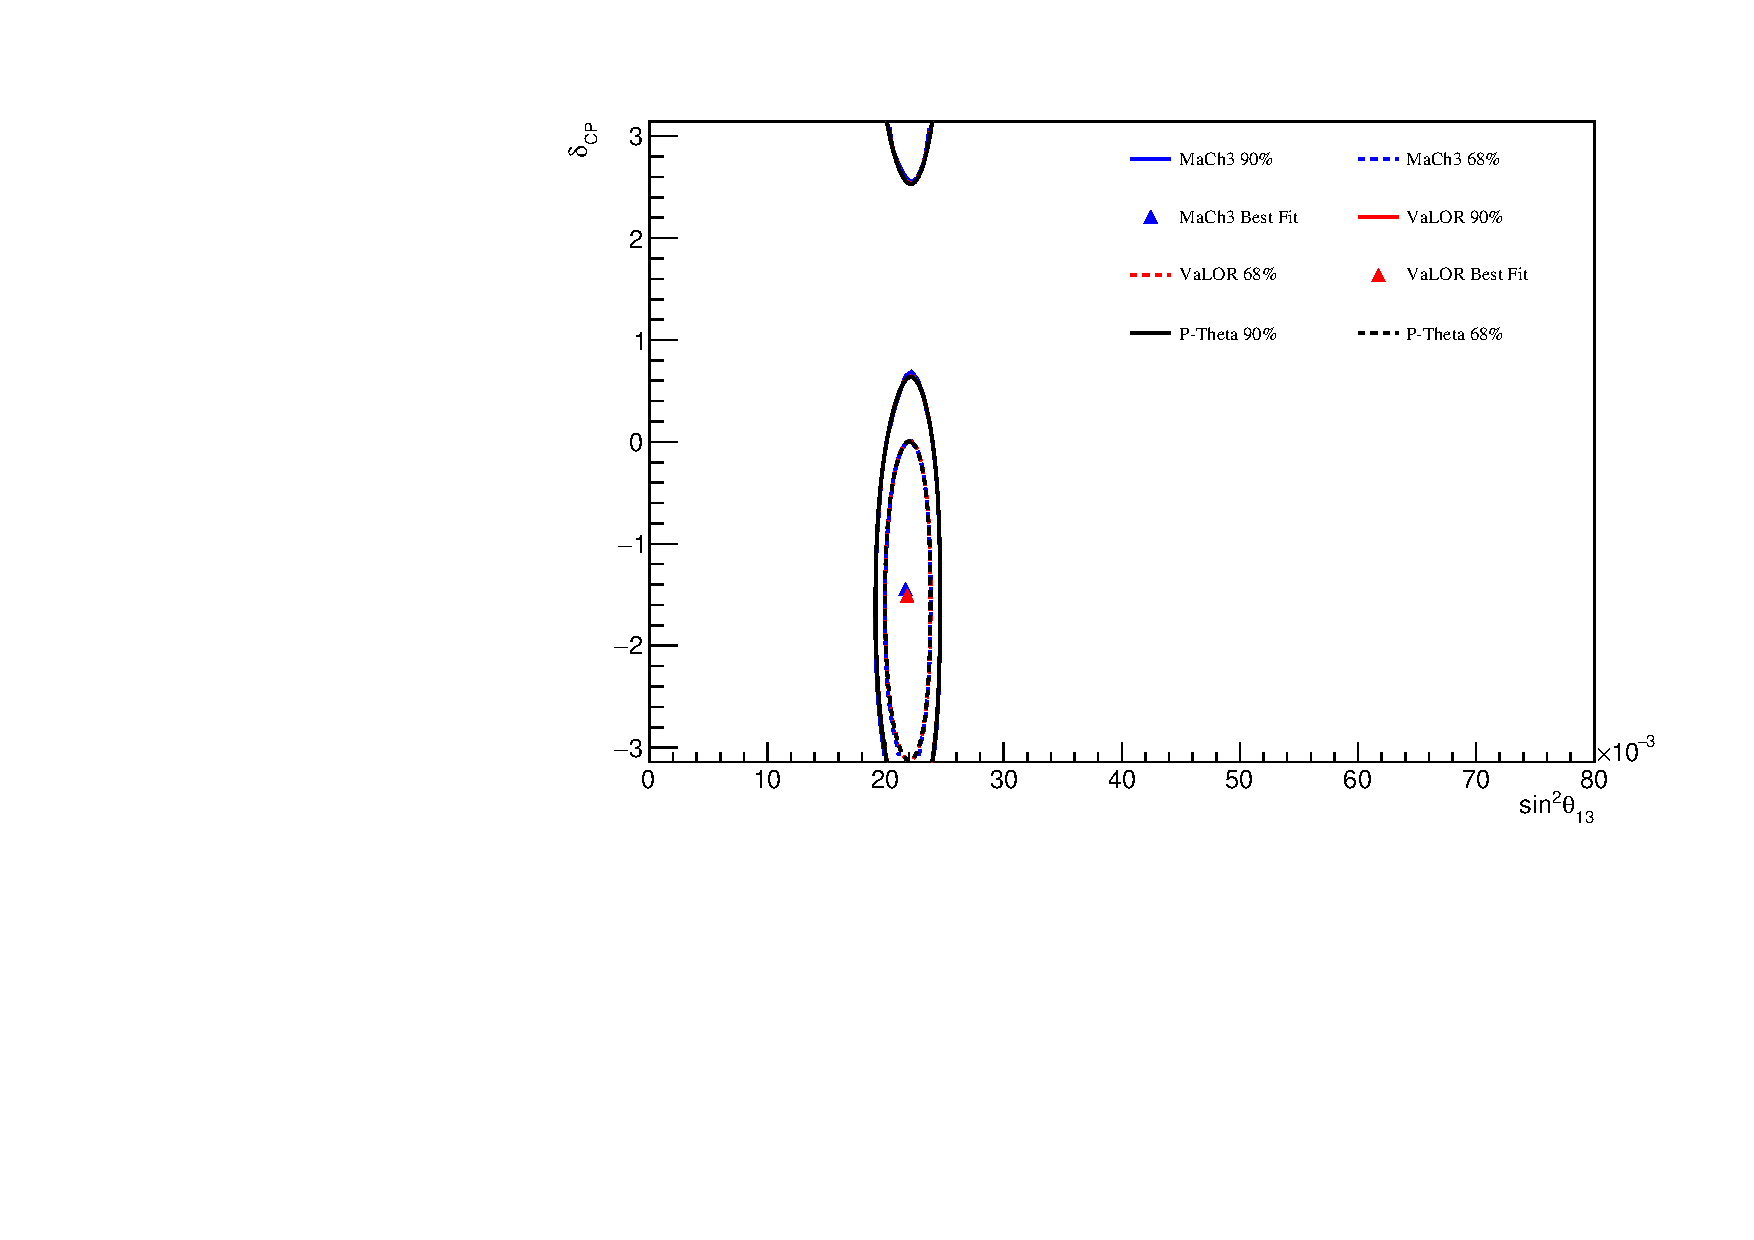
\includegraphics[width=.8\textwidth]{TalkPics/run17canalysescomparisons_210716/comparedcontours/comparedcontours_threeanalyses_th13dcp_IH.pdf}
  \end{frame}

  \begin{frame}
    \frametitle{Comparison of Asimov Set 1 1D contours}
    \centering
    \begin{columns}
      \column{.5\textwidth}
      \centering
      \large \textcolor{beamer@icmiddleblue}{NH}
      \column{.5\textwidth}
      \centering
      \large \textcolor{beamer@icmiddleblue}{IH}
    \end{columns}
    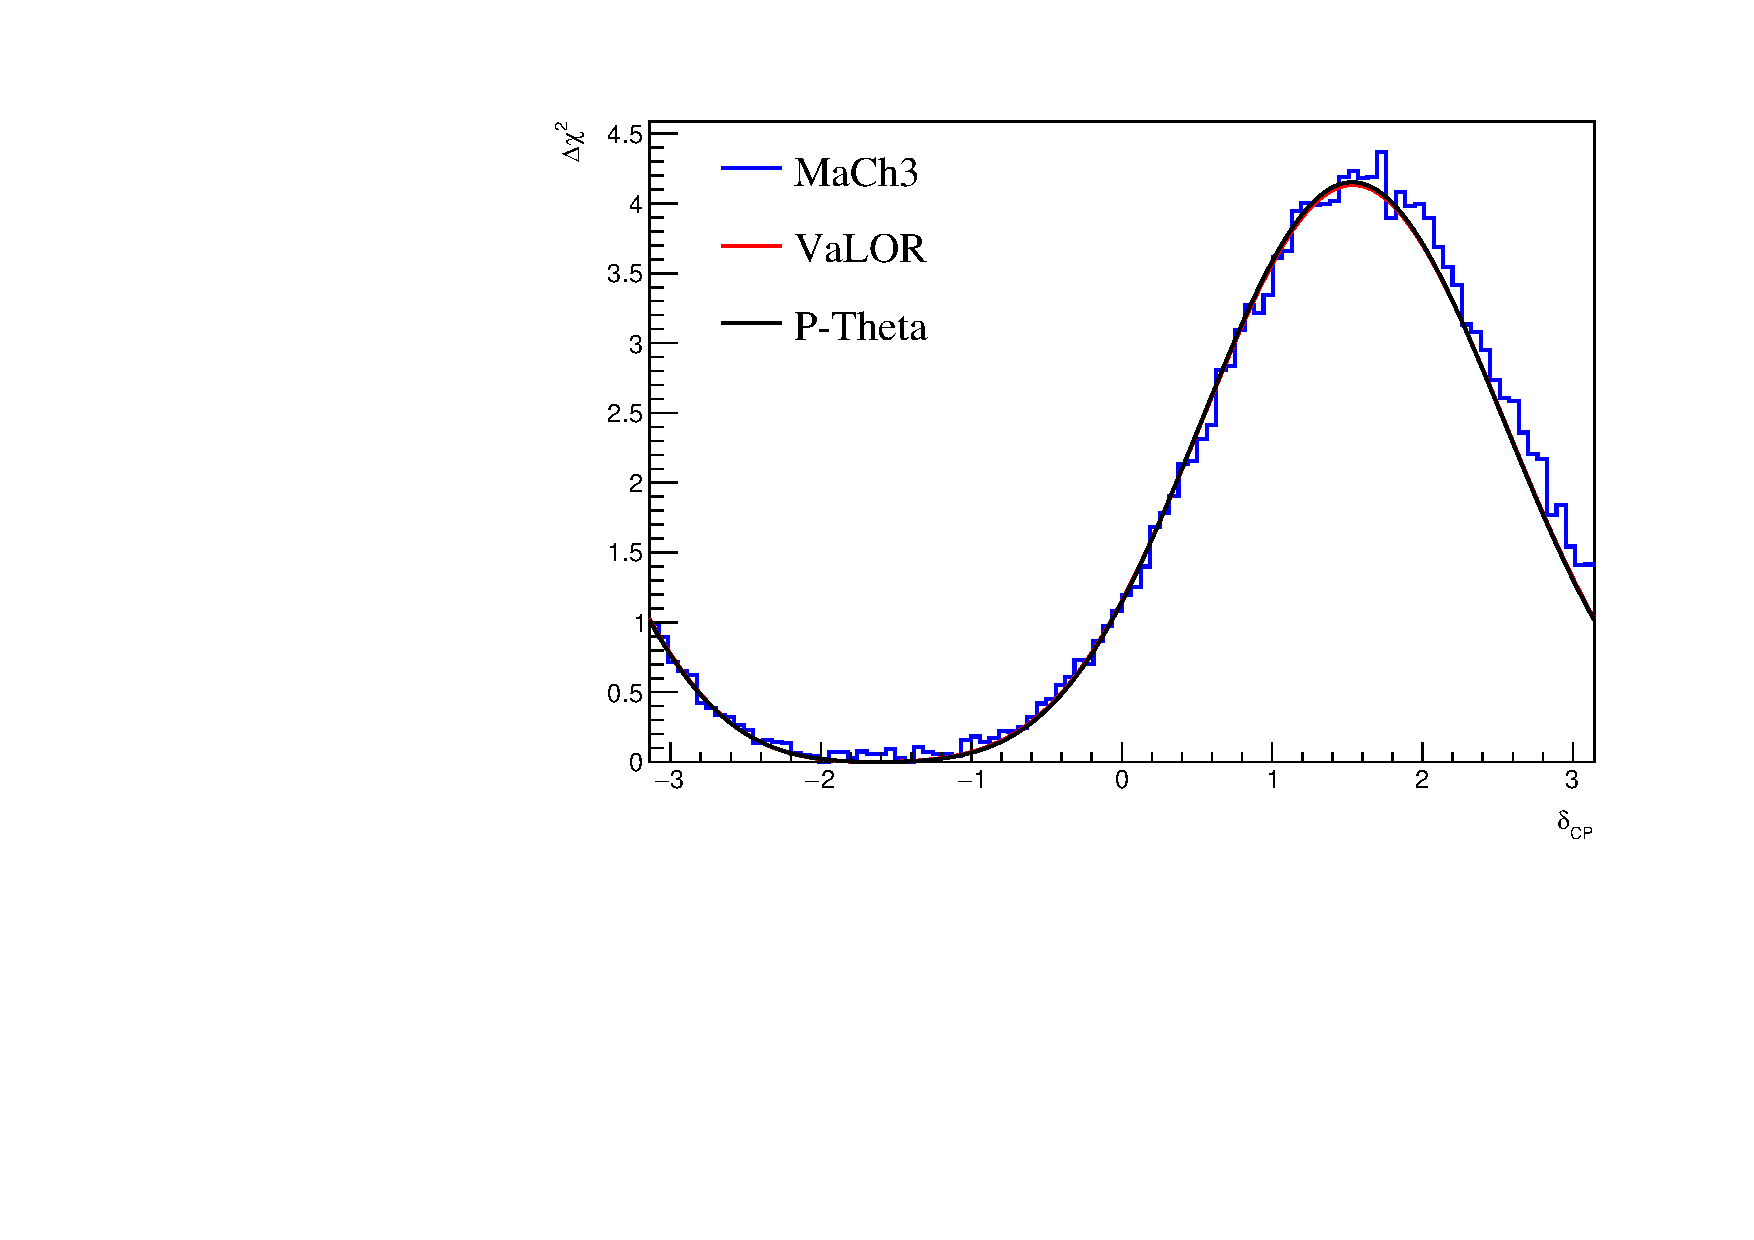
\includegraphics[width=.5\textwidth]{TalkPics/run17canalysescomparisons_210716/comparedcontours/comparedcontours_threeanalyses_dcp_NH.pdf}
    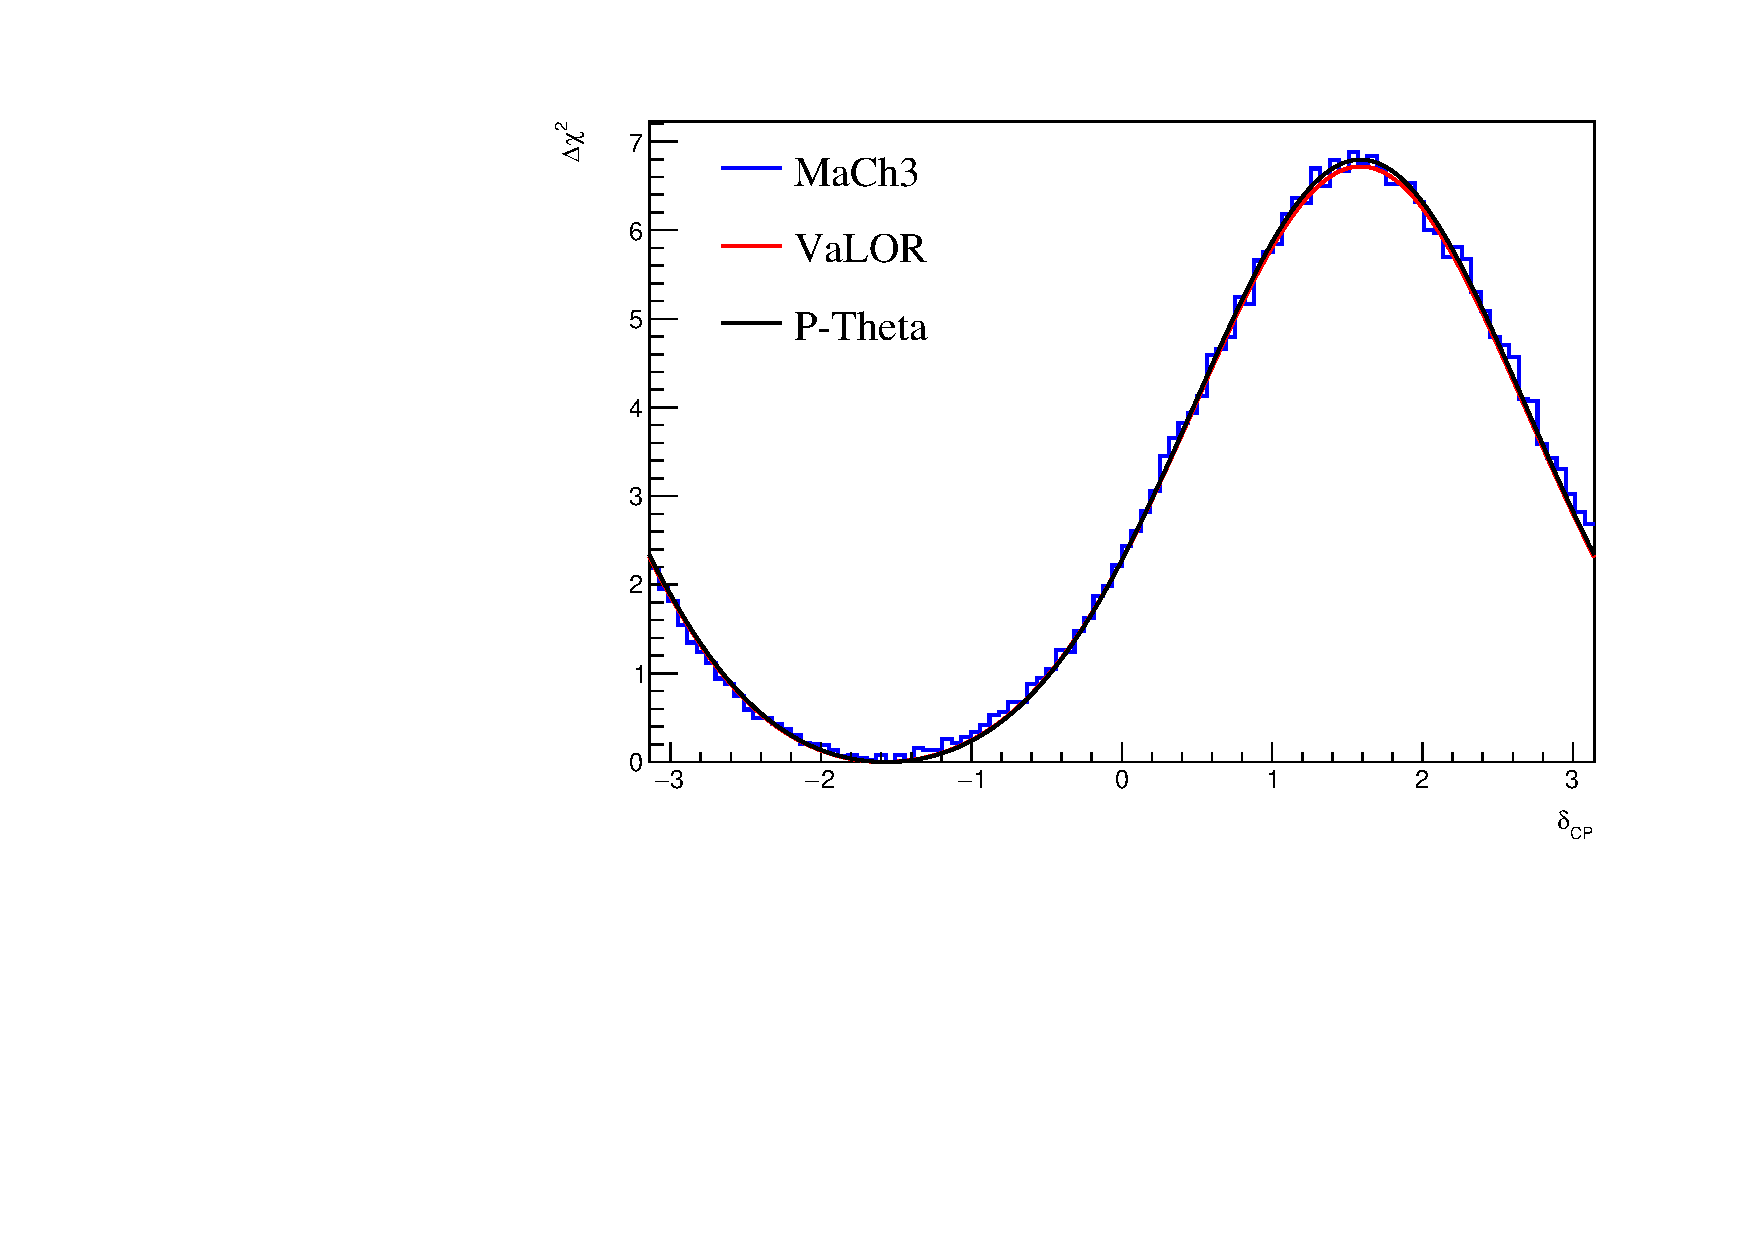
\includegraphics[width=.5\textwidth]{TalkPics/run17canalysescomparisons_210716/comparedcontours/comparedcontours_threeanalyses_dcp_IH.pdf}
  \end{frame}

  \begin{frame}
    \centering
    \huge \textcolor{beamer@icmiddleblue}{MaCh3 data fit results}
  \end{frame}

  %??Observed Rates

  \begin{frame}
    \frametitle{Observed rates}
    \begin{table}
       \centering
       \caption{Number of data events in each of the SK samples for run 1--7c, compared to the prefit MC prediction (using oscillation parameters set 1).}
        \begin{tabular}{ccccc}
         & FHC $\rm{1R_{\mu}}$ & FHC $\rm{1R_{e}}$ & RHC $\rm{1R_{\mu}}$ & RHC $\rm{1R_{e}}$ \\
            \hline
            Data          & 135       & 32       & 66        & 4     \\
            Prefit MC     & 136.21    & 28.75    & 64.40     & 6.01  \\
            \hline
            Data/MC Ratio & 1.00      & 1.11     & 1.02      & 0.67  \\
    \end{tabular}
    \end{table}
  \end{frame}

  \begin{frame}
    \frametitle{Observed spectra}
    \begin{columns}
      \column{.5\textwidth}
      \centering
      \large \textcolor{beamer@icmiddleblue}{$\nu$~mode $\rm{1R_{\mu}}$}
      \column{.5\textwidth}
      \centering
      \large \textcolor{beamer@icmiddleblue}{$\nu$~mode $\rm{1R_{e}}$}
      \end{columns}
    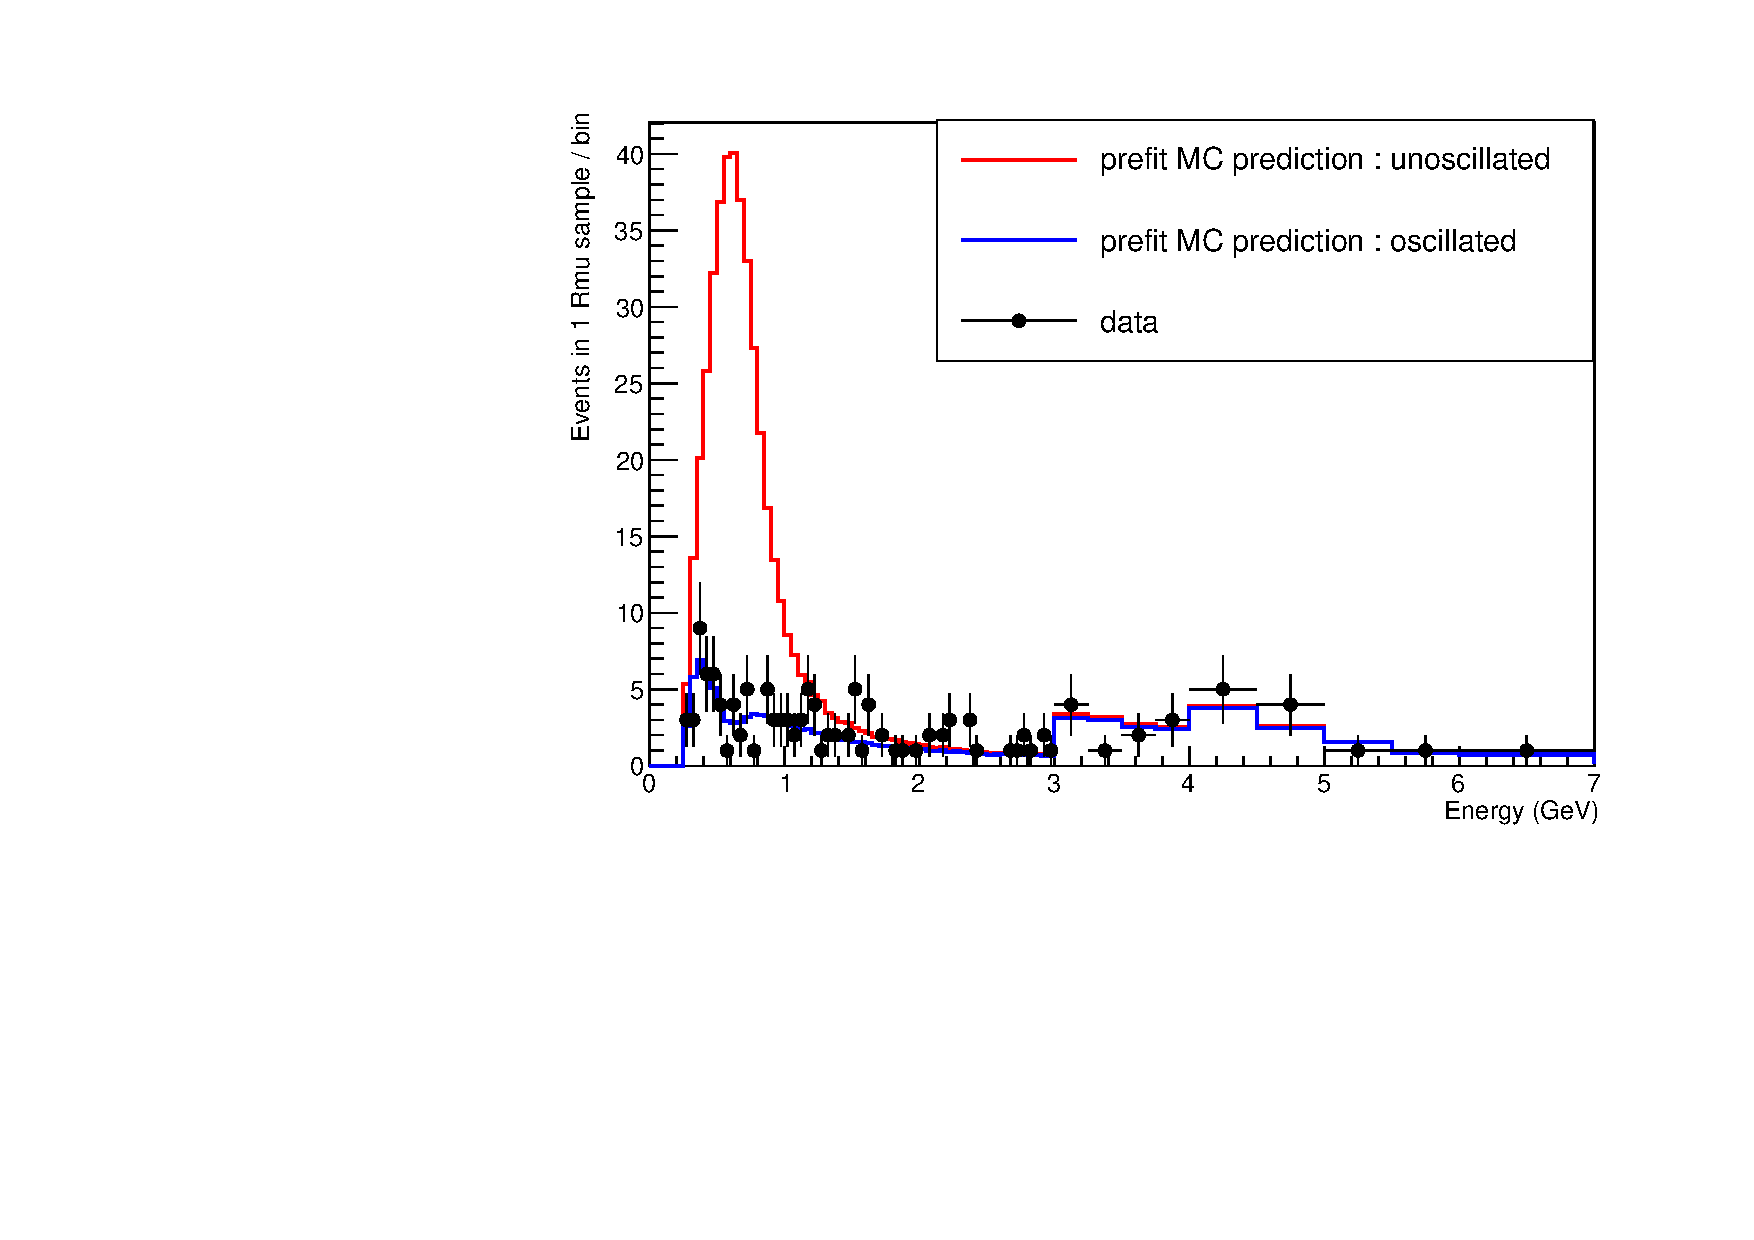
\includegraphics[width=.5\textwidth]{TalkPics/run17canalysescomparisons_210716/Run1-7update/run1-7c_mcpred/Run1-7c_newflux_nobanff_FHC_1Rmu.pdf}
    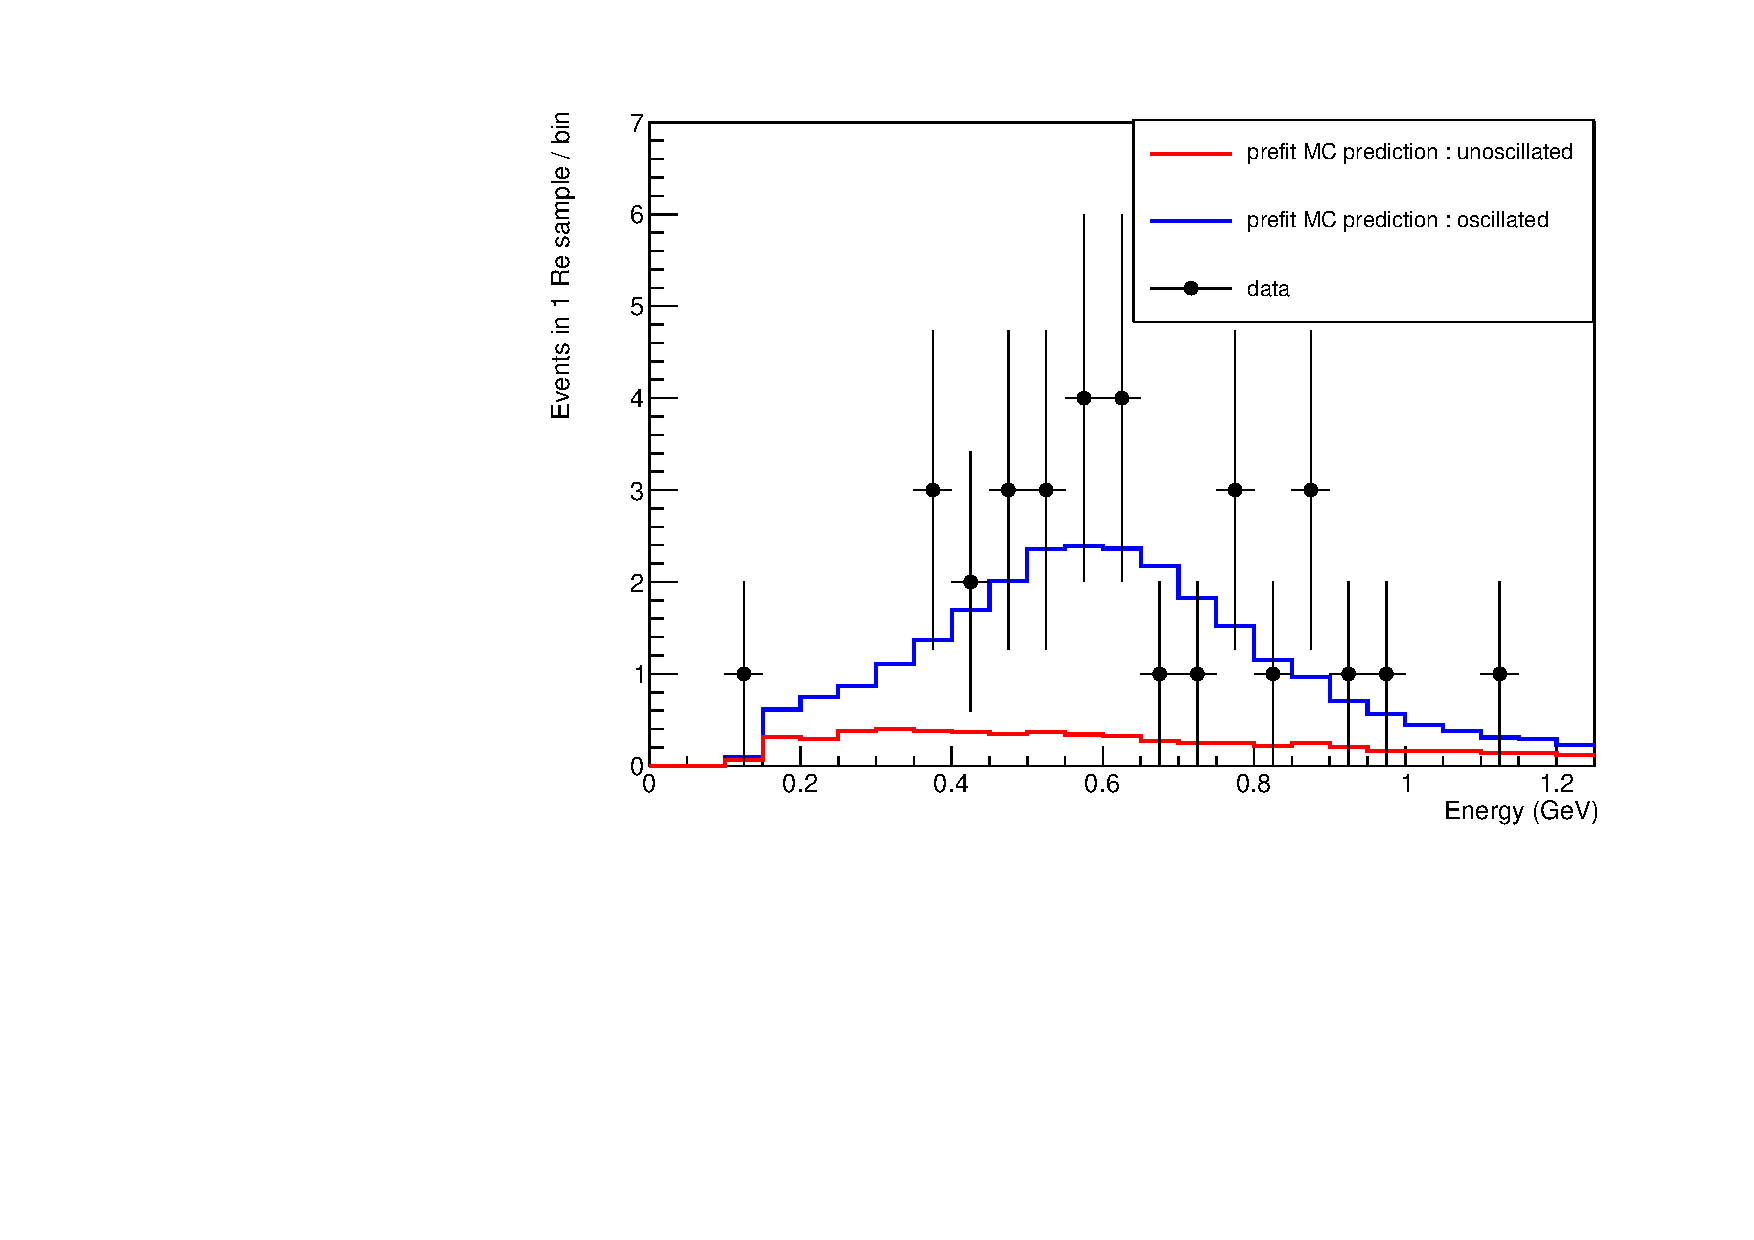
\includegraphics[width=.5\textwidth]{TalkPics/run17canalysescomparisons_210716/Run1-7update/run1-7c_mcpred/Run1-7c_newflux_nobanff_FHC_1Re.pdf}
  \end{frame}

  \begin{frame}
    \frametitle{Observed spectra}
    \begin{columns}
      \column{.5\textwidth}
      \centering
      \large \textcolor{beamer@icmiddleblue}{$\bar{\nu}$~mode $\rm{1R_{\mu}}$}
      \column{.5\textwidth}
      \centering
      \large \textcolor{beamer@icmiddleblue}{$\bar{\nu}$~mode $\rm{1R_{e}}$}
      \end{columns}
        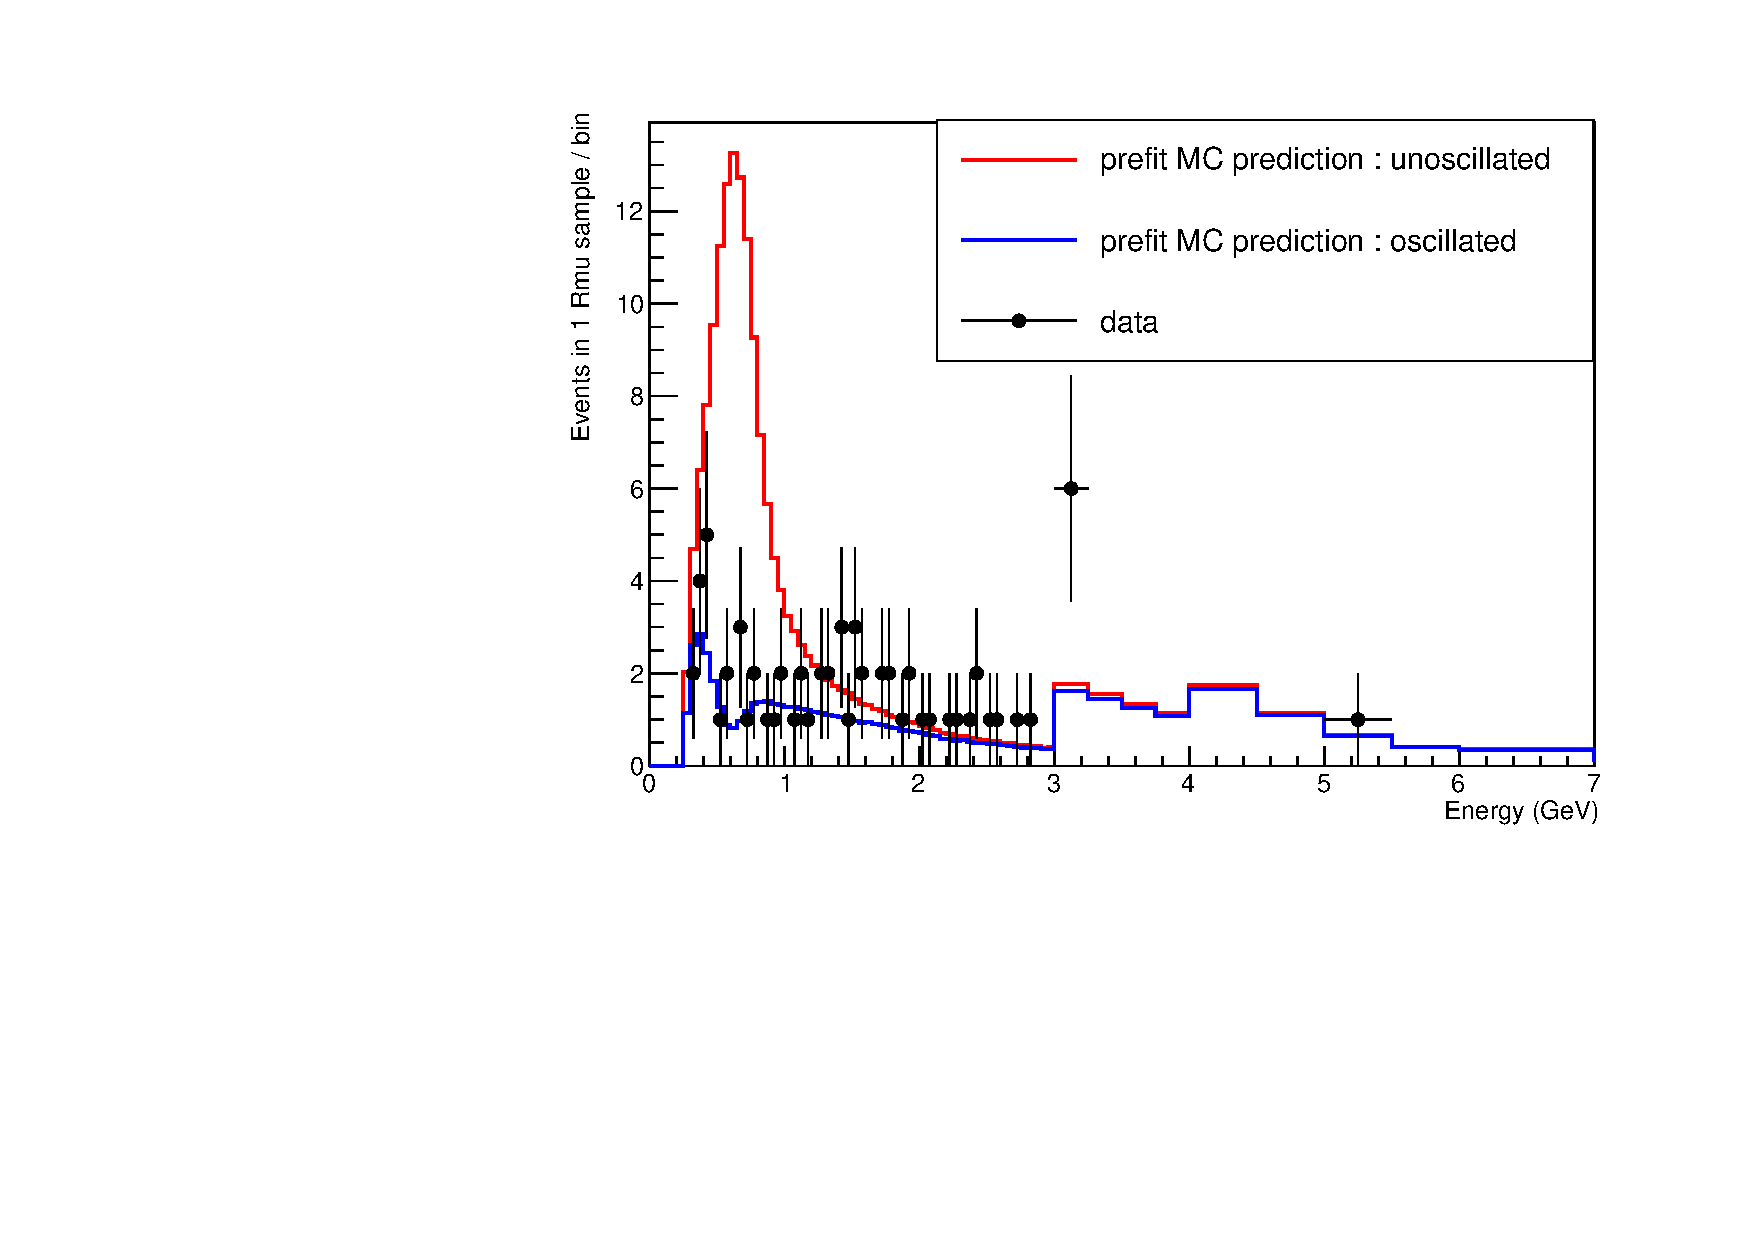
\includegraphics[width=.5\textwidth]{TalkPics/run17canalysescomparisons_210716/Run1-7update/run1-7c_mcpred/Run1-7c_newflux_nobanff_RHC_1Rmu.pdf}
        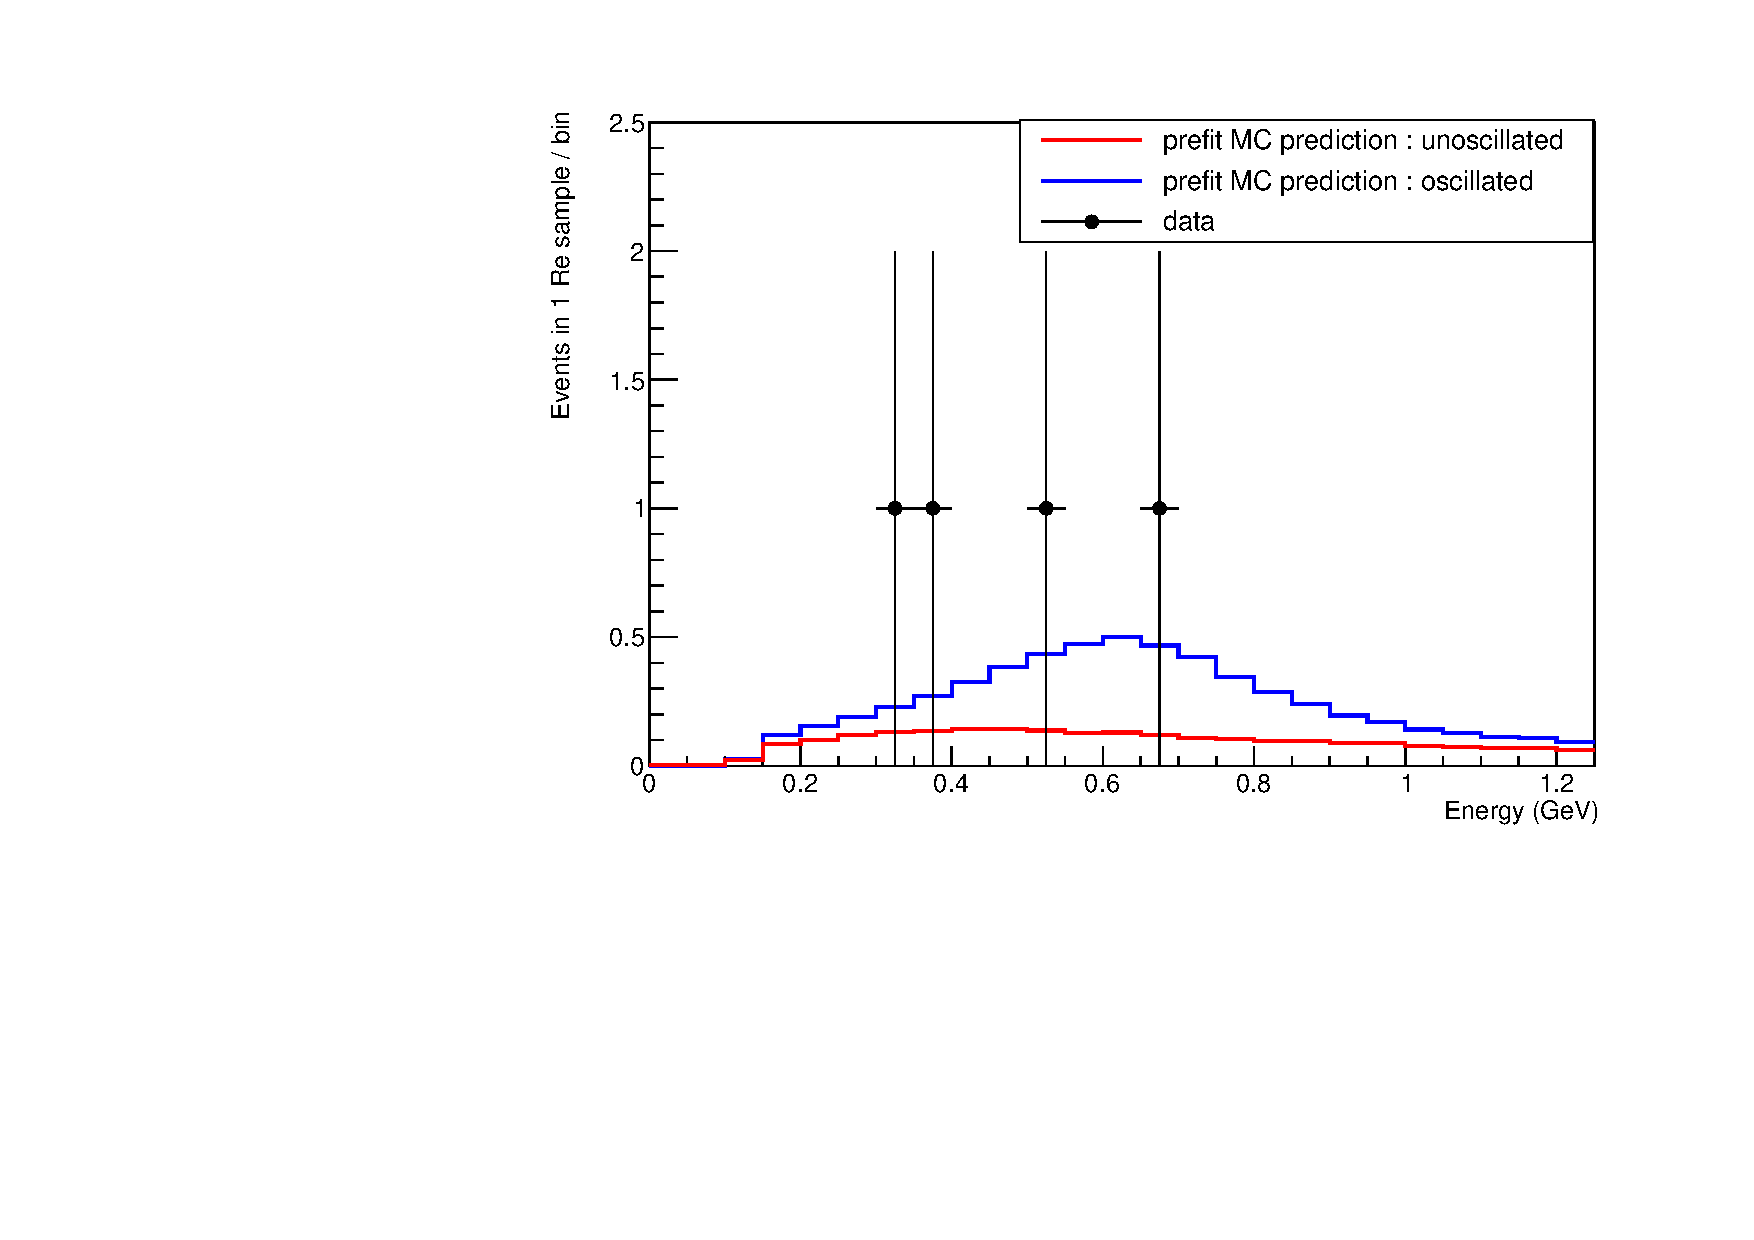
\includegraphics[width=.5\textwidth]{TalkPics/run17canalysescomparisons_210716/Run1-7update/run1-7c_mcpred/Run1-7c_newflux_nobanff_RHC_1Re.pdf}
  \end{frame}





  \begin{frame}
    \frametitle{MaCh3 data fit results}
    \centering
    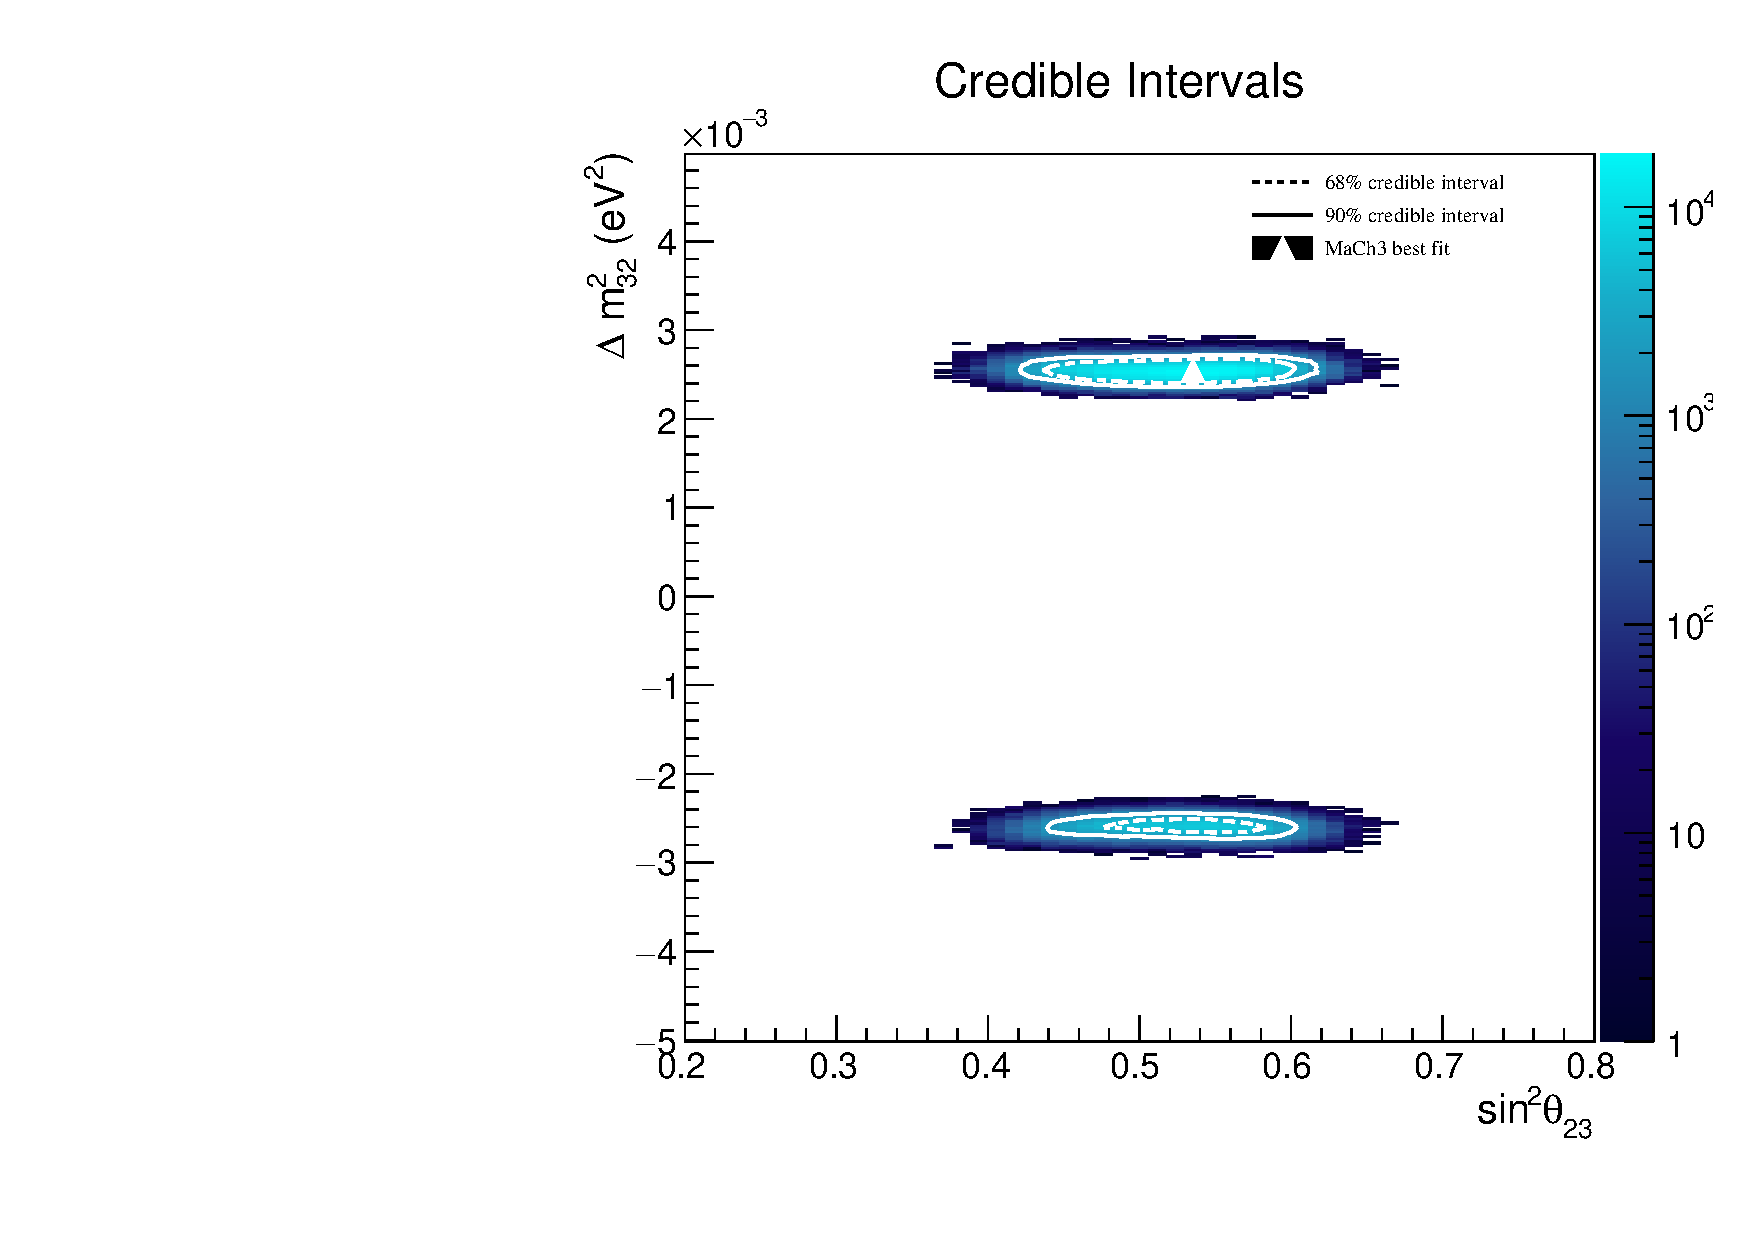
\includegraphics[width=.6\textwidth]{TalkPics/run17canalysescomparisons_210716/contours_wRC_datafit/contours_th23dm23_both.pdf}
  \end{frame}

  \begin{frame}
    \frametitle{MaCh3 data fit results}
    \centering
    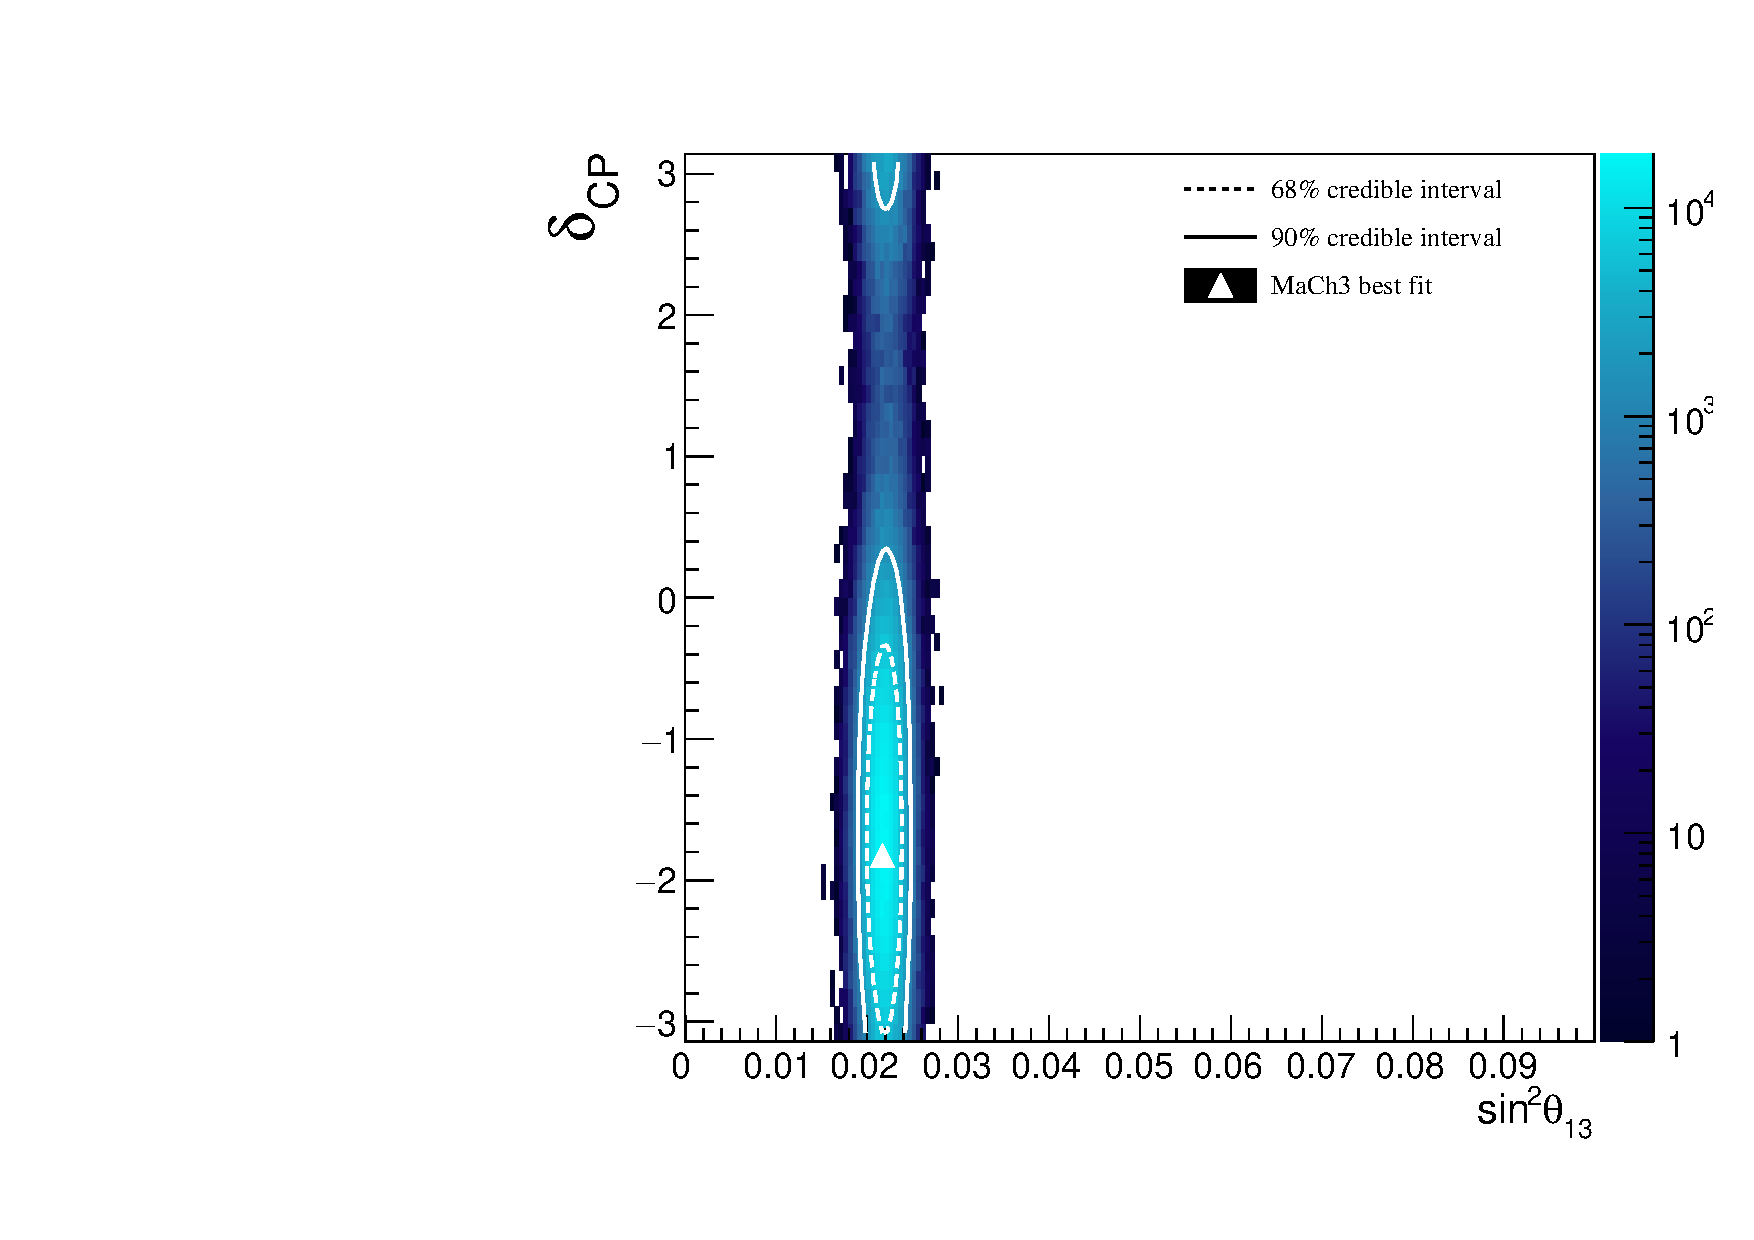
\includegraphics[width=.6\textwidth]{TalkPics/run17canalysescomparisons_210716/contours_wRC_datafit/contours_th13dcp_both.pdf}
  \end{frame}

  \begin{frame}
    \frametitle{MaCh3 data fit results}
    \centering
    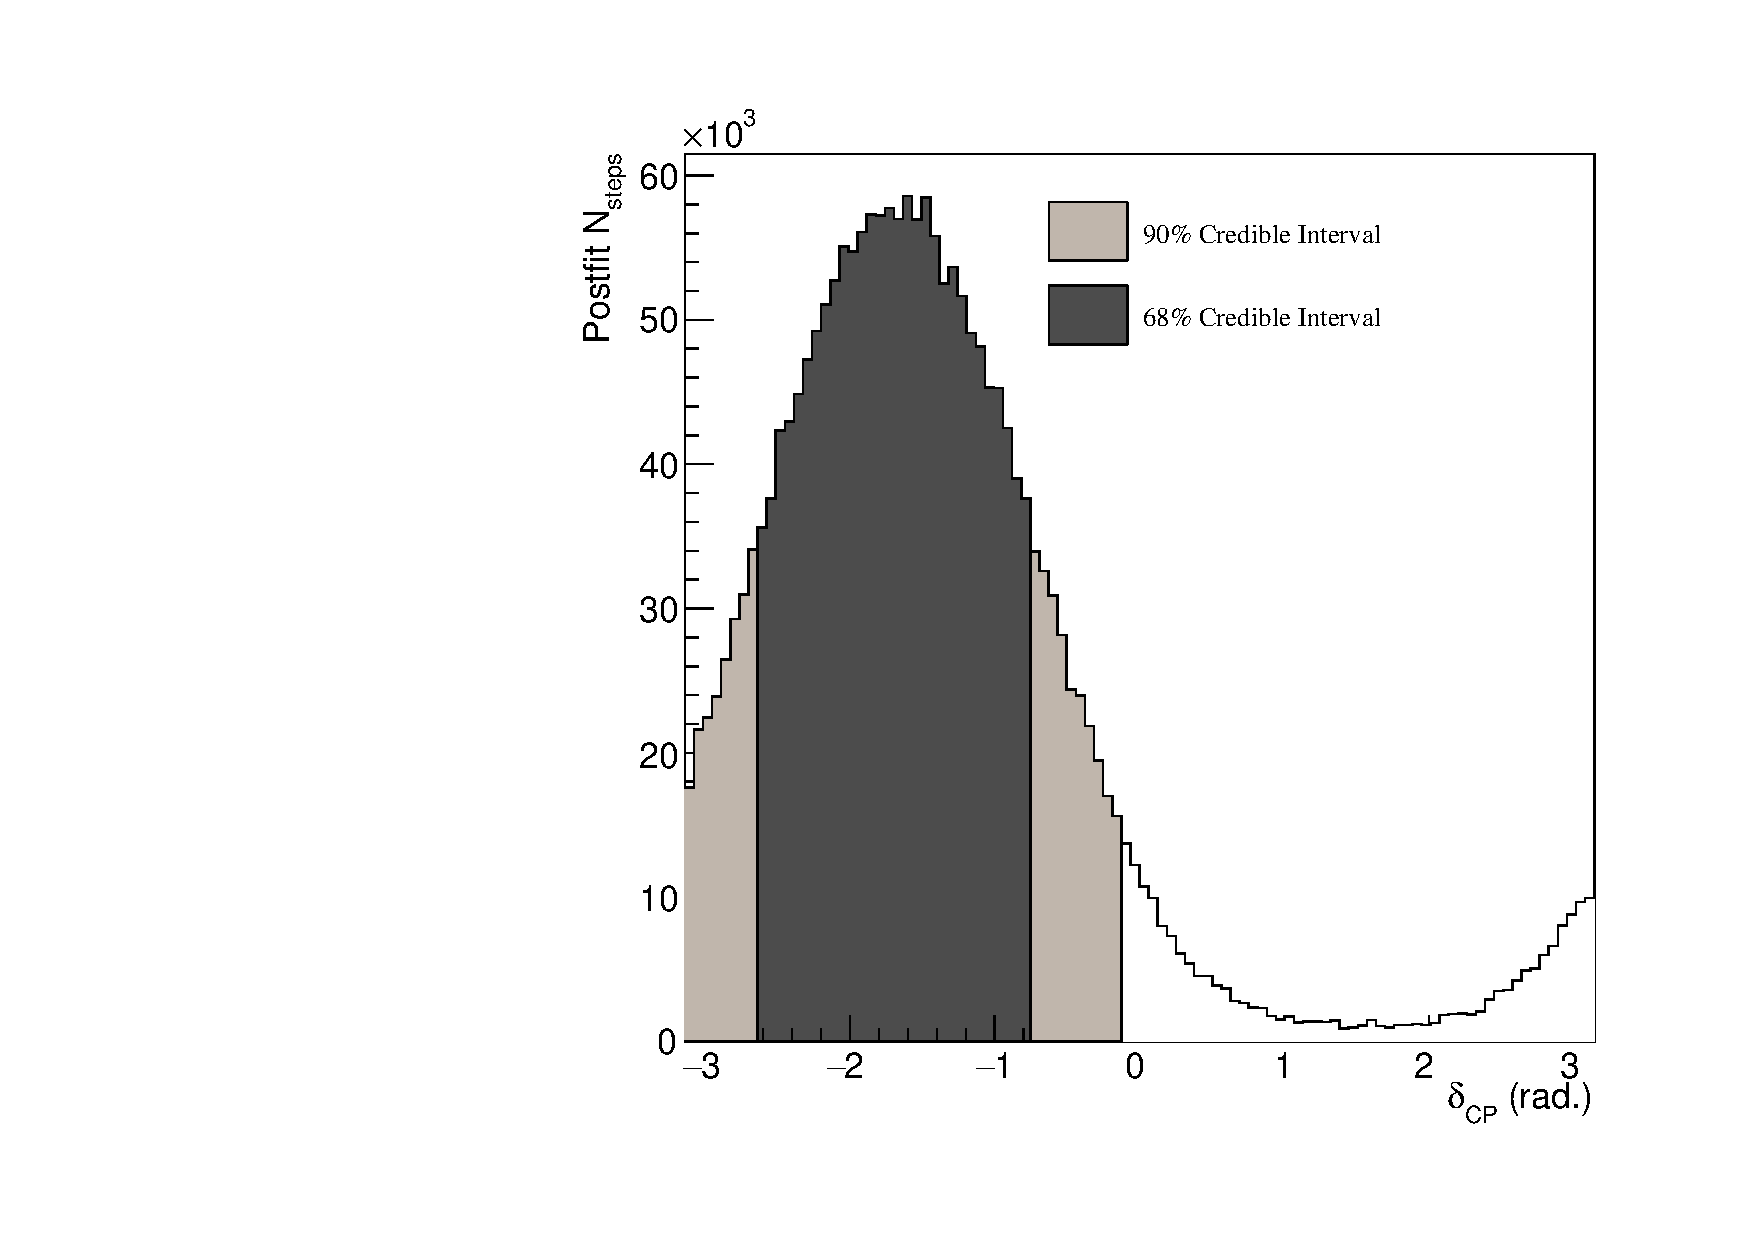
\includegraphics[width=.6\textwidth]{TalkPics/run17canalysescomparisons_210716/contours_wRC_datafit/contours_1D_dcp_both.pdf}
  \end{frame}

  \begin{frame}
    \centering
    \huge \textcolor{beamer@icmiddleblue}{VaLOR-MaCh3 data fit comparison}
  \end{frame}

  \begin{frame}
    \frametitle{Comparison of Data 2D contours - NH}
    \centering
    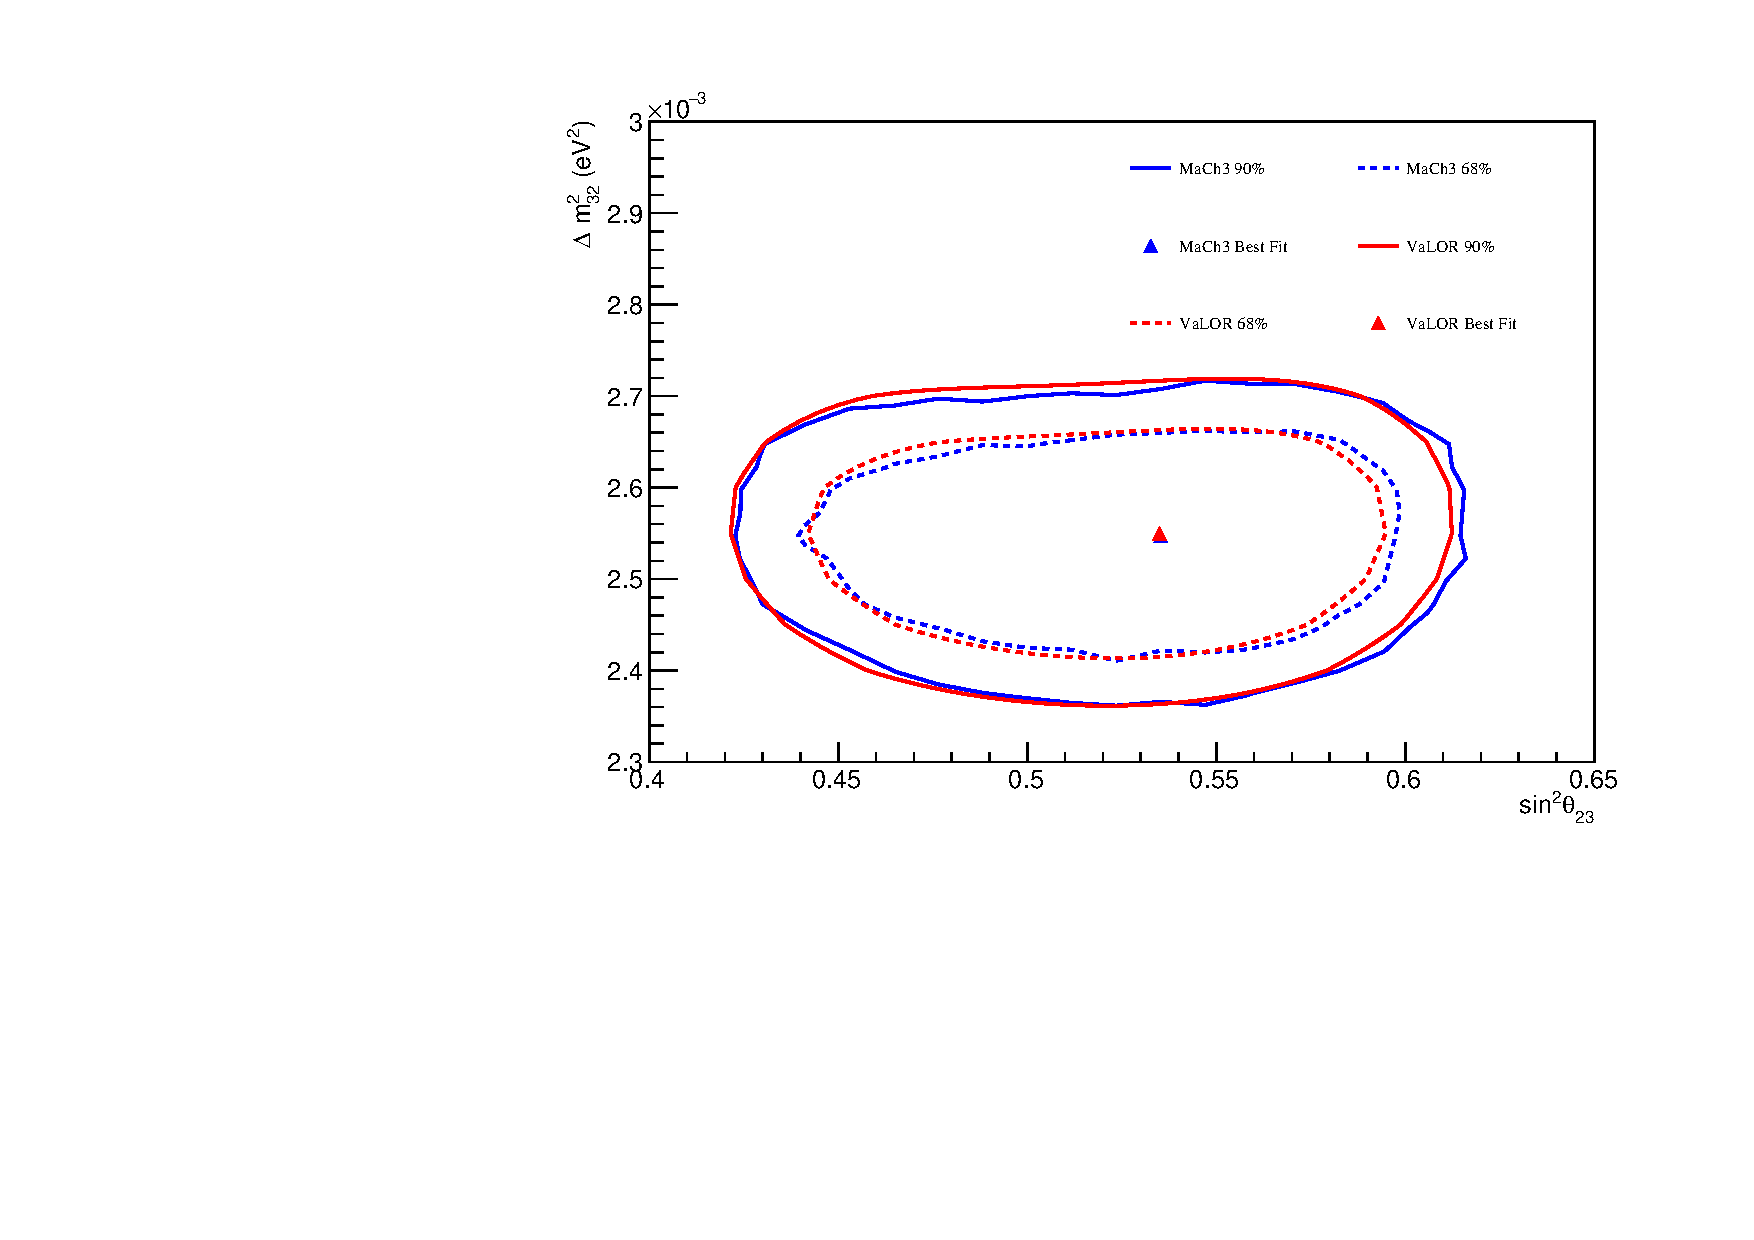
\includegraphics[width=.8\textwidth]{TalkPics/run17canalysescomparisons_210716/comparedcontours_data/comparedcontours_threeanalyses_NH.pdf}
  \end{frame}

  \begin{frame}
    \frametitle{Comparison of Data 2D contours - IH}
    \centering
    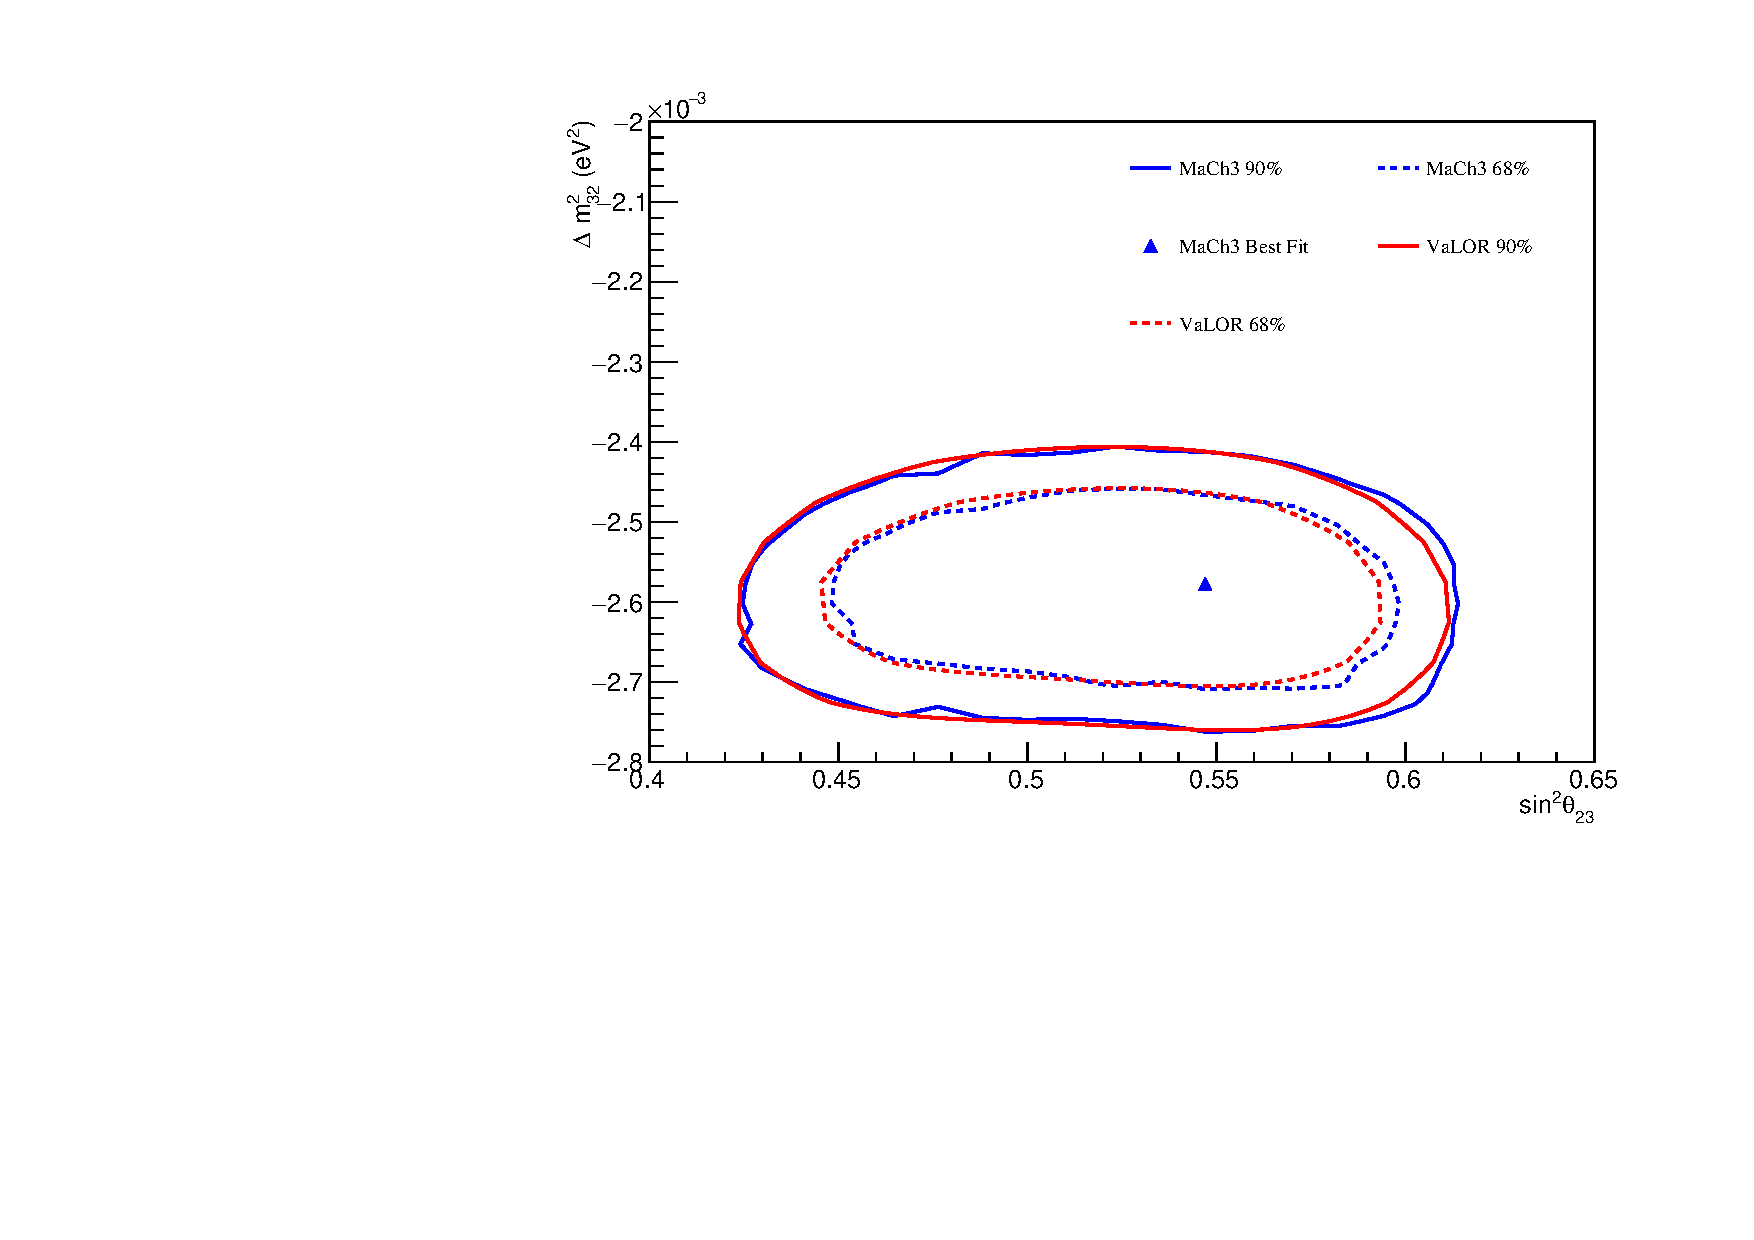
\includegraphics[width=.8\textwidth]{TalkPics/run17canalysescomparisons_210716/comparedcontours_data/comparedcontours_threeanalyses_IH.pdf}
  \end{frame}

  \begin{frame}
    \frametitle{Comparison of Data 2D contours - NH}
    \centering
    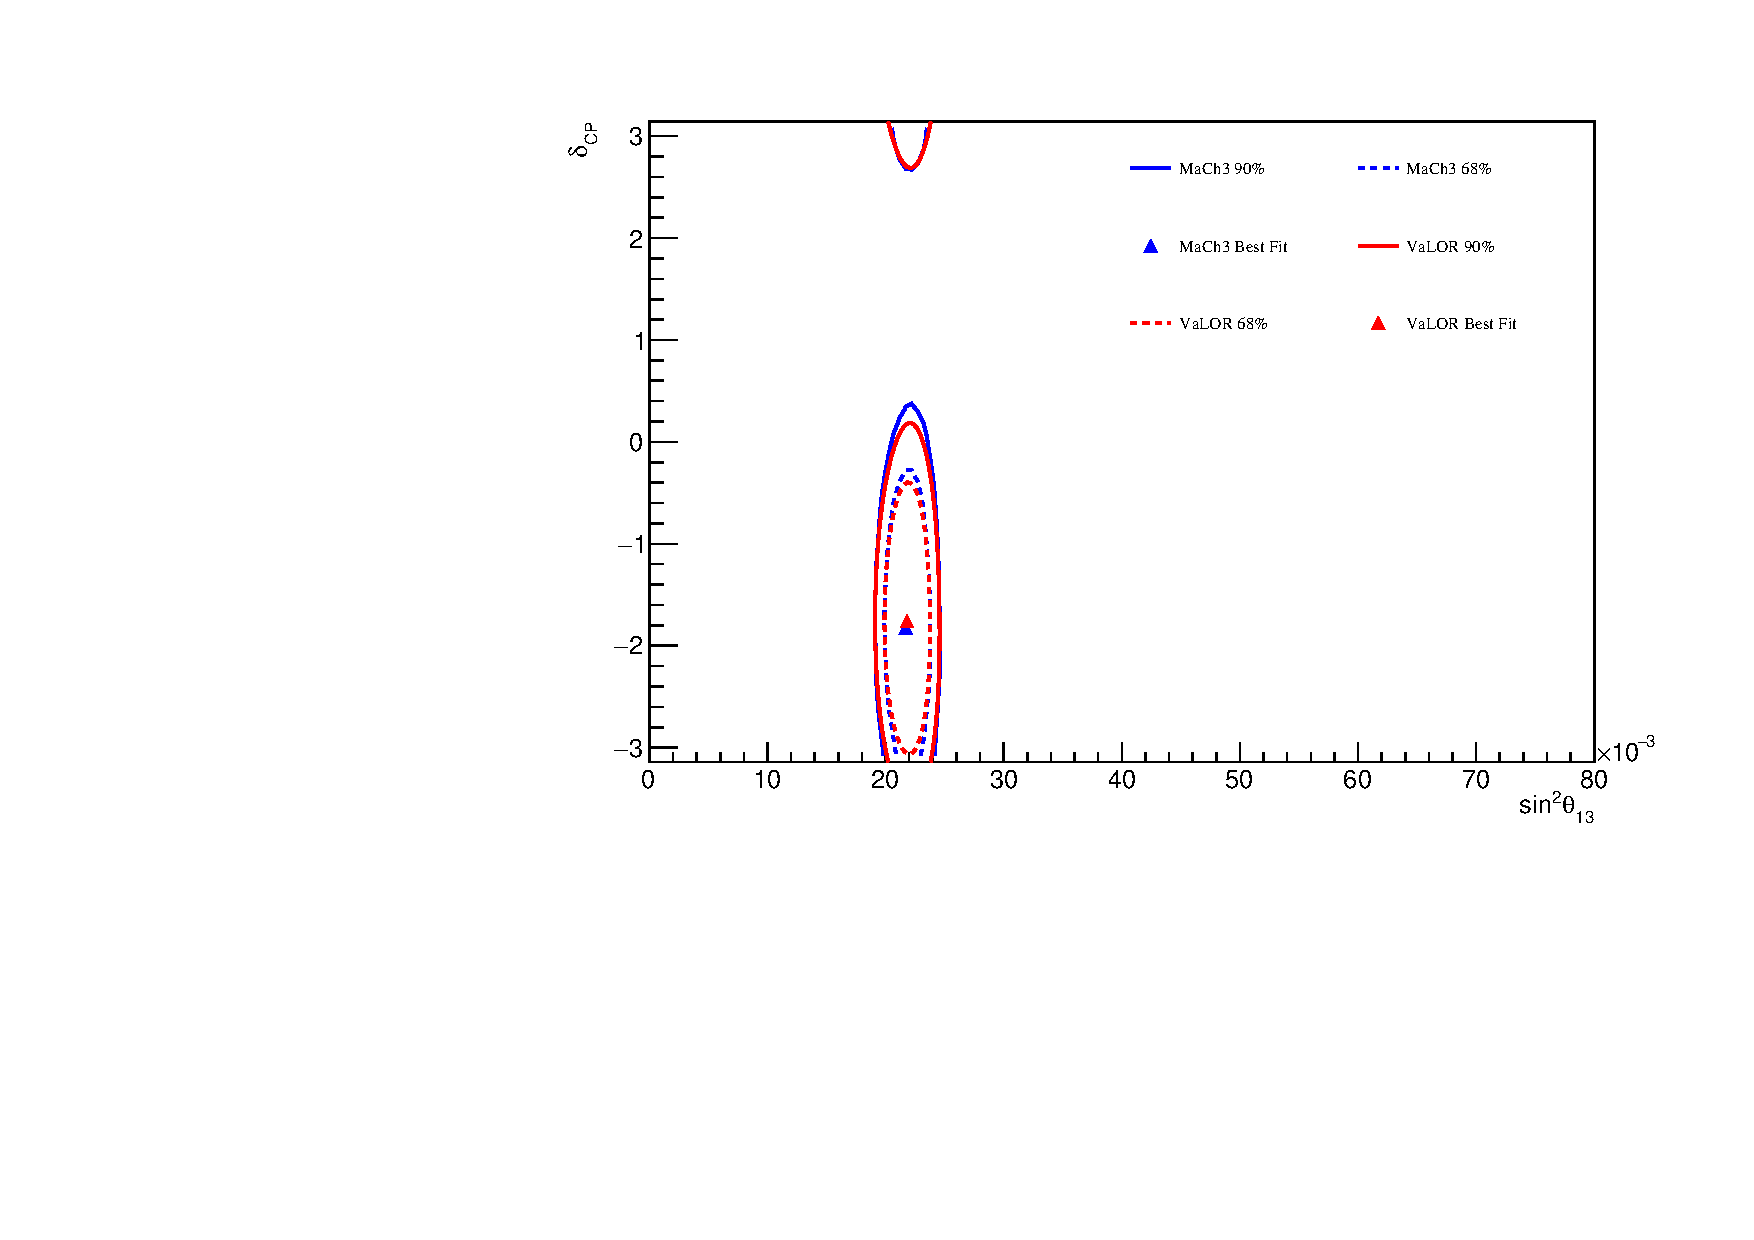
\includegraphics[width=.8\textwidth]{TalkPics/run17canalysescomparisons_210716/comparedcontours_data/comparedcontours_threeanalyses_th13dcp_NH.pdf}
  \end{frame}

  \begin{frame}
    \frametitle{Comparison of Data 2D contours - IH}
    \centering
    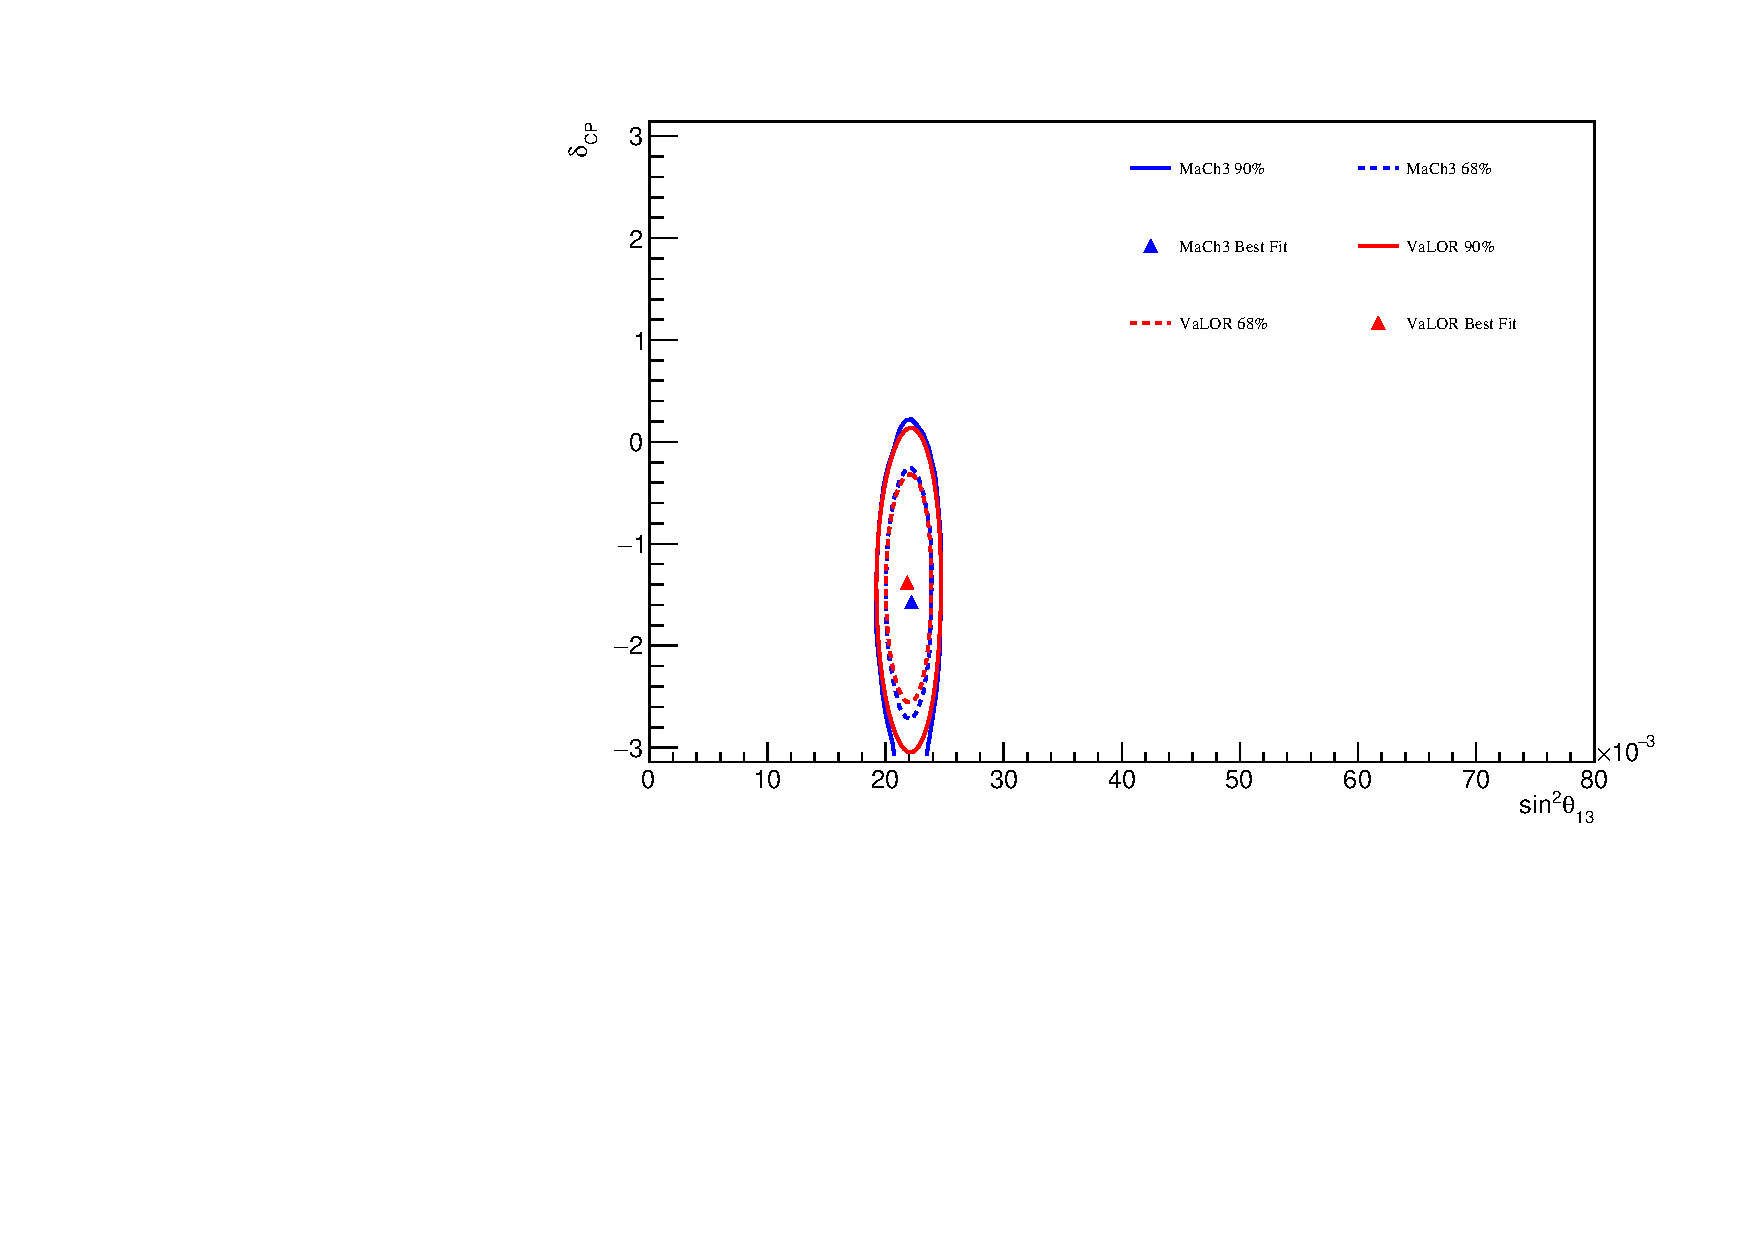
\includegraphics[width=.8\textwidth]{TalkPics/run17canalysescomparisons_210716/comparedcontours_data/comparedcontours_threeanalyses_th13dcp_IH.pdf}
  \end{frame}

  \begin{frame}
    \frametitle{Comparison of Data 1D contours}
    \centering
    \begin{columns}
      \column{.5\textwidth}
      \centering
      \large \textcolor{beamer@icmiddleblue}{NH}
      \column{.5\textwidth}
      \centering
      \large \textcolor{beamer@icmiddleblue}{IH}
    \end{columns}
    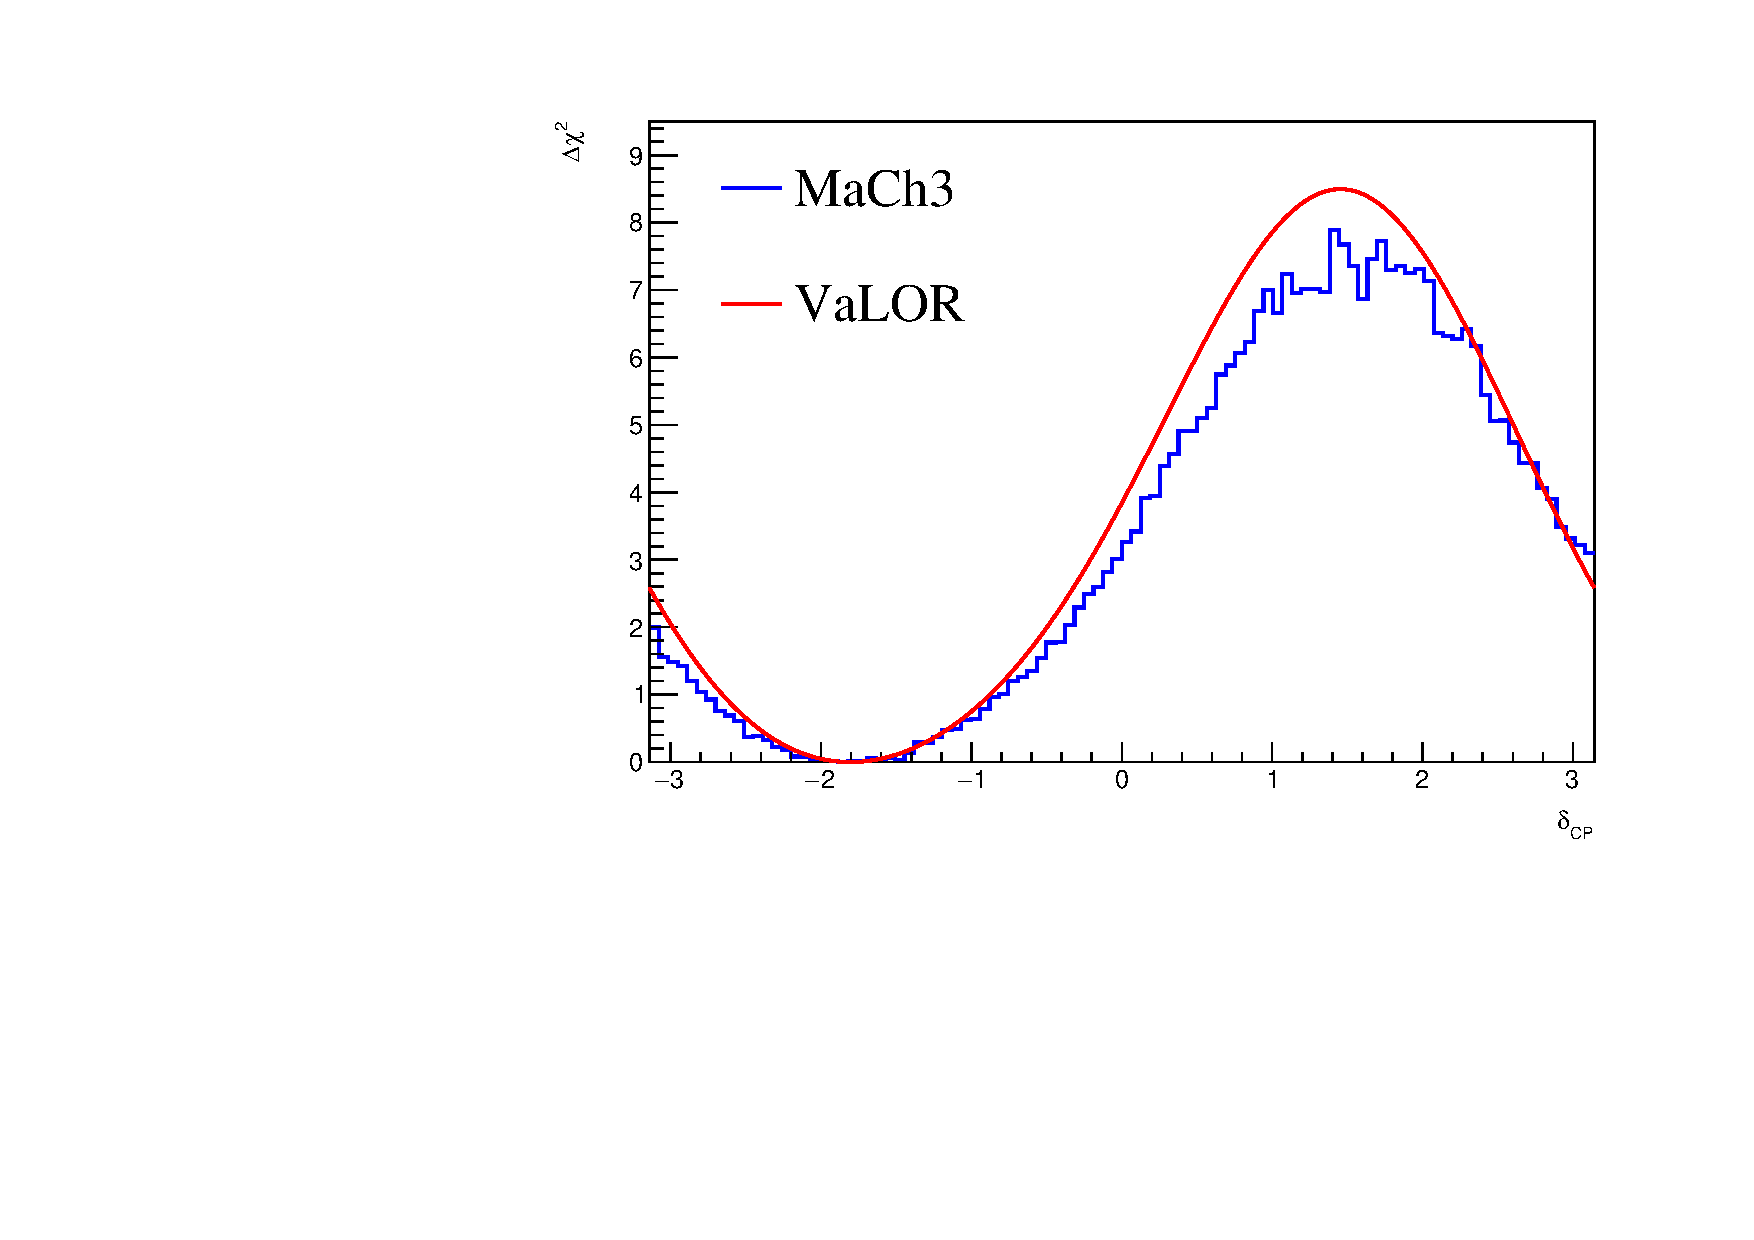
\includegraphics[width=.5\textwidth]{TalkPics/run17canalysescomparisons_210716/comparedcontours_data/comparedcontours_threeanalyses_dcp_NH.pdf}
    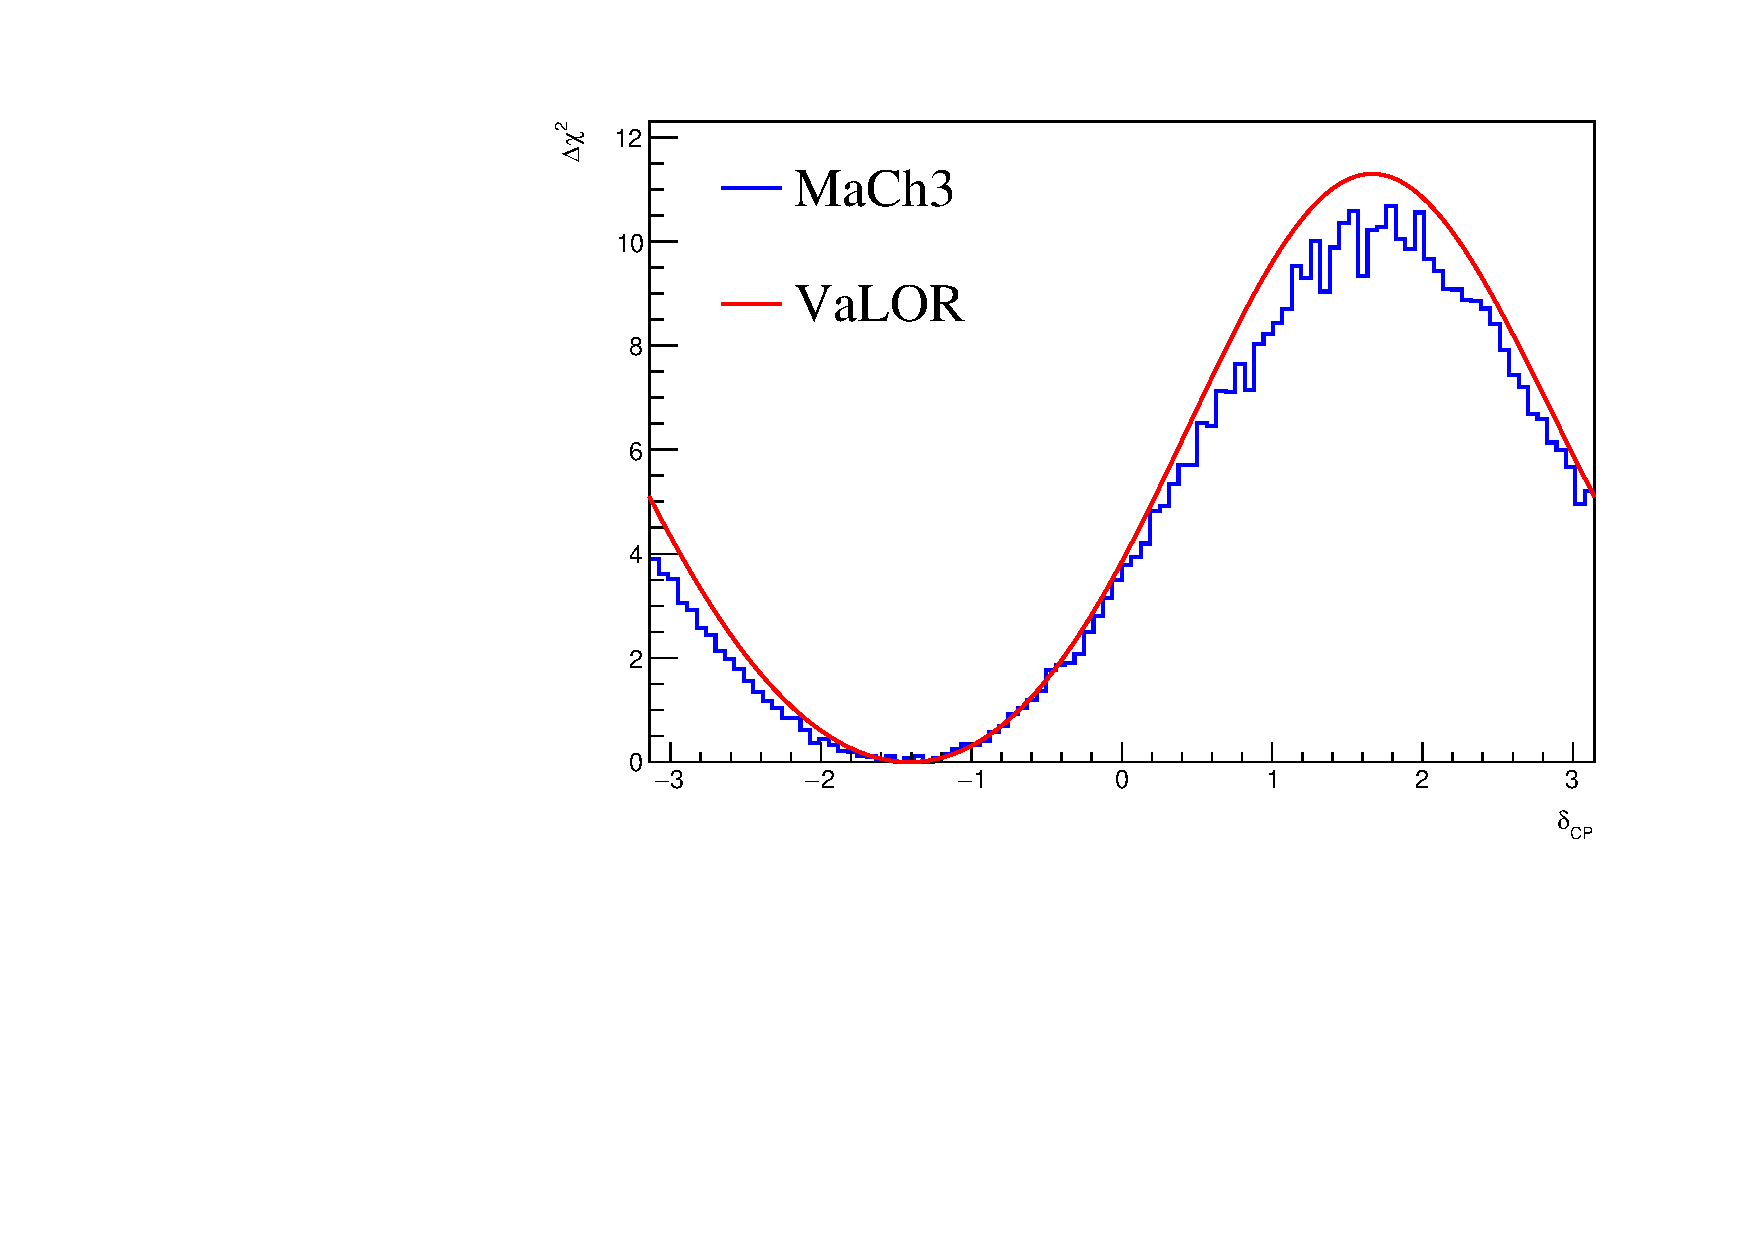
\includegraphics[width=.5\textwidth]{TalkPics/run17canalysescomparisons_210716/comparedcontours_data/comparedcontours_threeanalyses_dcp_IH.pdf}
  \end{frame}


  \begin{frame}
    \frametitle{}
    \label{lastframe}
    \begin{block}{}
      \begin{itemize}
      \item 2D and 1D Asimov contours compared between all three analyses
      \item[-] Agreement between analyses is good
      \item Data results have been shown
      \item[-] Similar differences between MaCh3 and VaLOR as in 1-7b seen
      \item[-] Expected to be due to $E_{rec}$ vs $E_{rec}-\theta$ binning
      \item[-] MaCh3 are working on implementing $E_{rec}-\theta$ binning
      \item Still working on results without reactor constraint and updating TN
      \end{itemize}
    \end{block}
  \end{frame}

  %Backup goes here
  
\end{fmffile}
\end{document}

